\documentclass[11pt,a4paper,oneside]{memoir}

\chapterstyle{section}
\copypagestyle{centerruled}{ruled}
\makeevenfoot{centerruled}{}{\thepage}{}
\makeoddfoot{centerruled}{}{\thepage}{}
\makeevenhead{centerruled}{}{}{\leftmark}
\makeoddhead{centerruled}{}{}{\leftmark}

\usepackage{graphicx}
\usepackage{geometry}
\usepackage{hyperref}
\usepackage[table]{xcolor}
\usepackage[backend=biber,style=numeric,maxnames=4,urldate=long]{biblatex}
\usepackage{tabularx}
\usepackage{acro}
\usepackage{amsmath}
\usepackage{amssymb}
\usepackage{caption}
\usepackage{subcaption}
\usepackage{algorithm}
\usepackage{algpseudocode}

\newcolumntype{L}{>{\raggedright\arraybackslash}X}
\newcolumntype{C}{>{\centering\arraybackslash}X}
\def\tabularxcolumn#1{m{#1}}

\addbibresource{bibliography.bib}

\hypersetup{
	colorlinks=true,
	linkcolor=black,
	urlcolor=blue,
	citecolor=black,
}

\graphicspath{{figures/}}

\setsecnumdepth{subsection}

\setcounter{tocdepth}{2}

\acsetup{make-links,list/display=all}

\DeclareAcronym{sw}{
	short=SW,
	long=Software,
}

\DeclareAcronym{hw}{
	short=HW,
	long=Hardware,
}

\DeclareAcronym{fsm}{
	short=FSM,
	long=Finite-State Machine,
}

\DeclareAcronym{hdl}{
	short=HDL,
	long=\acl{hw} Description Language,
}

\DeclareAcronym{rtl}{
	short=RTL,
	long=Register-Transfer Level
}

\DeclareAcronym{hls}{
	short=HLS,
	long=High-Level Synthesis,
}

\DeclareAcronym{fpga}{
	short=FPGA,
	long=Field-Programmable Gate Array,
}

\DeclareAcronym{fifo}{
	short=FIFO,
	long=First-In First-Out,
}

\DeclareAcronym{lru}{
	short=LRU,
	long=Least Recently Used,
}

\DeclareAcronym{ram}{
	short=RAM,
	long=Random Access Memory,
	long-plural-form=Random Access Memories,
}

\DeclareAcronym{dram}{
	short=DRAM,
	long=Dynamic RAM,
}

\DeclareAcronym{bram}{
	short=BRAM,
	long=Block RAM,
}

\DeclareAcronym{axi}{
	short=AXI,
	long=Advanced eXtensible Interface,
}

\DeclareAcronym{raw}{
	short=RAW,
	long=Read After Write,
}

\DeclareAcronym{ii}{
	short=II,
	long=Initiation Interval,
}

\DeclareAcronym{l1}{
	short=L1,
	long=Level 1,
}

\DeclareAcronym{l2}{
	short=L2,
	long=Level 2,
}

\DeclareAcronym{api}{
	short=API,
	long=Application Programming Interface,
}

\DeclareAcronym{ipc}{
	short=IPC,
	long=Inter-Process Communication,
}

\DeclareAcronym{lsb}{
	short=LSB,
	long=Least Significant Bit,
}

\DeclareAcronym{msb}{
	short=MSB,
	long=Most Significant Bit,
}

\DeclareAcronym{dsp}{
	short=DSP,
	long=Digital Signal Processor,
}

\DeclareAcronym{lut}{
	short=LUT,
	long=Lookup Table,
}

\DeclareAcronym{ff}{
	short=FF,
	long=Flip-Flop,
}

\DeclareAcronym{cc}{
	short=CC,
	long=Clock Cycle,
}

\renewcommand*{\maketitle}%
{
	\newgeometry{left=2cm,right=2cm,top=3cm,bottom=3.5cm}

	\begin{center}
		\begingroup
		{\Huge\textbf{POLITECNICO DI TORINO}}\\[\baselineskip]
		\rule{\textwidth}{2pt}\par
		\vspace*{1em}
		{\LARGE\textbf{Master's Degree in Computer Engineering}}\\[\baselineskip]
		\vspace*{1em}
		{\Large\textbf{Master's Degree Thesis}}\\
		\vspace*{2cm}
		{\huge\textbf{Acceleration by Separate-Process Cache for
		Memory-Intensive Algorithms on \acs{fpga} via \acl{hls}}}\\
		\vspace*{1cm}
		
\includegraphics[width=.3\textwidth]{figures/polito-logo}
	\end{center}
	\vfill
	\begin{minipage}{0.4\textwidth}
		\begin{flushleft}
			{\Large
				\textbf{Supervisor}\\
				Prof.\ Luciano Lavagno
			}
		\end{flushleft}
	\end{minipage}
	\begin{minipage}{0.4\textwidth}
		\begin{flushright} 
			{\Large
				\textbf{Candidate}\\
				Giovanni Brignone\\
				ID: 274148
			}
		\end{flushright}
	\end{minipage}  
	\vspace*{2cm}
	\begin{center}
		{\Large\textbf{Academic year 2020-2021}}
	\end{center}
	\endgroup

	\restoregeometry 
}

\begin{document}
\pagestyle{empty}
\maketitle

\clearpage
\pagestyle{plain}

\frontmatter
\chapter*{Abstract}
The end of the Moore's Law validity is making the performance advance of
\acl{sw} run on general purpose processors more challenging than ever.
Since current technology cannot scale anymore it is necessary to approach the
problem from a different point of view: application-specific \acl{hw} can
provide higher performance and lower power consumption, while requiring higher
design efforts and higher deployment costs.

The problem of the high design efforts can be mitigated by the \acf{hls}, since
it helps improve designer productivity thanks to convenient \acl{sw}-like
tools.

The problem of high deployment costs can be tackled with \acp{fpga}, which allow
implementing special-purpose \acl{hw} modules on general-purpose underlying
physical architectures.

\bigskip
One of the open issues of \ac{hls} is the memory bandwidth bottleneck which
limits performance, especially critical in case of memory-bound algorithms.

\acp{fpga} memory system is composed of three main kinds of resources: registers,
\aclp{bram} and external \acsp{dram}.
Current \ac{hls} tools allow exploiting this memory hierarchy manually, in a
scratchpad-like fashion: the objective of this thesis work is to automate the
memory management by providing an easily integrable and fully customizable cache
system for \ac{hls}.

\bigskip
The proposed implementation has been developed using Vitis\texttrademark HLS
tool by Xilinx Inc..

The first development phase produced a single-port cache module, in the form of
a C++ class configurable through templates in terms of number of sets, ways,
words per line and replacement policy.
The cache lines have been mapped to \acp{bram}.
To obtain the desired performance, an unconventional (for \ac{hls}) multiprocess
architecture has been developed: the cache module is a separate process with
respect to the algorithm using it: the algorithm logic sends a memory access
request to the cache and reads its response, communicating through \acsp{fifo}.

\bigskip
In the second development phase, the focus was put on performance optimization,
in two dimensions: increasing the memory hierarchy depth by introducing a
\ac{l1} cache and increasing parallelism by enabling multiple ports.

The \ac{l1} cache is composed of cache logic inlined in the user algorithm: this
solution allows to cut the costs of \acp{fifo} communications. To keep \ac{l1}
cache simple it has been implemented with a write-through write policy,
therefore it provides advantages for read accesses only. It is configurable in
the number of lines and each line contains the same number of words of the
associated \ac{l2} cache.

The multi-port solution provides a single \ac{l2} cache accessible from multiple
\acp{fifo} ports, each of which can be associated with a dedicated \ac{l1}
cache.
It is possible to specify the number of ports through a template parameter and
it typically corresponds to the unrolling factor of the loop in which the cache
is accessed.

\bigskip
In order to evaluate performance and resource usage impact of the developed
cache module, multiple algorithms with different memory access patterns have
been synthesized and simulated, with all data accessed to \ac{dram} (performance
lower bound), to \ac{bram} (performance higher bound) and to cache (with
multiple configurations).

\vfill
\pagebreak

\tableofcontents*
\vfill
\pagebreak

\listoffigures
\vfill
\pagebreak

\listoftables
\vfill
\pagebreak

\printacronyms[heading=chapter,name={List of Acronyms}]
\vfill
\pagebreak

\clearpage
\pagestyle{centerruled}

\mainmatter
\chapter{Background}
The literature about cache systems, the \acl{hls} state of the art and an
analysis of the resources available on board modern \acp{fpga} are the
fundamental background for this thesis work.

\section{Cache}
Memory devices are crucial components of computing systems as they can pose a
higher bound in terms of performance, especially when executing memory-intensive
algorithms.
The ideal memory should be fast, large and cheap, but current technology forces
the designer to choose a trade-off between the metrics.

A common solution to this problem is to set up a memory hierarchy in
which fast but small memories are paired with large but slow memories, which
allows getting good performance on average while containing costs.

This hierarchy can be managed by two main approaches:
\begin{itemize}
	\item \emph{Scratchpad}: different memories belongs to different
		addressing spaces: the user is in charge of manually choosing
		what memory to access: this approach allows to optimally
		exploit the hierarchy at the cost of high design effort.
	\item \emph{Cache}: different memories belongs to the same addressing
		space: the system automatically uses the whole hierarchy,
		exploiting spatial locality (accessed data is likely physically
		close to previously accessed data) and temporal locality
		(accessed data has likely recently been accessed), which are
		typical of many algorithms.
\end{itemize}

\subsection{Structure}
A cache memory is logically split into \emph{sets} containing \emph{lines} (or
\emph{ways}) which are in turn made up of \emph{words}, as shown in
Figure~\ref{fig:cache_logic_structure}.

\begin{figure}[!htb]
	\centering
	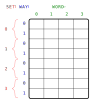
\includegraphics[width=.5\textwidth]{cache_logic_structure}
	\caption{Cache logic structure.}
	\label{fig:cache_logic_structure}
\end{figure}

Whenever a word $w$ is requested, there are two possibilities:
\begin{itemize}
	\item \emph{Hit}: $w$ is present in the cache: the request can be
		immediately fulfilled.
	\item \emph{Miss}: $w$ is not present in the cache: it is necessary to
		retrieve it from lower level memory before fulfilling the
		request.
\end{itemize}
During the data retrieving, a cache line is filled with a block of contiguous
words loaded from the lower level memory, trying to exploit spatial locality of
future accesses, while mapping policies and replacement policies determine which
cache line to overwrite, trying to exploit temporal locality.

If the cache memory is writable, data consistency is ensured by a consistency
policy.
\subsection{Policies}
\subsubsection{Mapping policy}
The mapping policy is in charge of statically associating a lower level memory
line to a cache set.

The \emph{set associative} policy is the most common mapping policy: given a
cache memory with $s$ sets of $w$ words, the word address (referred to the lower
level memory) bits are split into three parts (as shown in
Figure~\ref{fig:address_partitioning}):
\begin{enumerate}
	\item $\log_2(w)$: offset of the word in the line.
	\item $\log_2(s)$: set.
	\item Remaining \acsp{msb}: tag identifying the specific line.
\end{enumerate}

\begin{figure}[!htb]
	\centering
	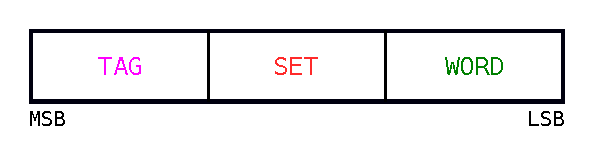
\includegraphics[width=.5\textwidth]{address_partitioning}
	\caption{Set associative policy address bits meaning.}
	\label{fig:address_partitioning}
\end{figure}

Special cases of this policy are:
\begin{itemize}
	\item \emph{Direct mapped} policy: each set is composed of a single
		line: the set bits identify a specific cache line, therefore
		there is no need for a replacement policy.
	\item \emph{Fully associative} policy: there is only a single set,
		therefore the line is fully determined by the replacement
		policy.
\end{itemize}

\subsubsection{Replacement policy}
The replacement policy is in charge of dynamically associating a lower level
memory line to a cache line of a set.

Multiple solutions of this problem have been developed, trying to maximize
the temporal locality exploitation.
Among the most commonly used solutions there are:
\begin{itemize}
	\item \emph{\acl{fifo}}: the line to be replaced is the first
		one that has been inserted to the cache.
	\item \emph{\acl{lru}}: the line to be replaced is the one
		that has least recently been accessed.
\end{itemize}

\subsubsection{Consistency policy}
The consistency policy is in charge of ensuring data consistency between
memories belonging to different hierarchy levels.

The most common solutions to this problem are:
\begin{itemize}
	\item \emph{Write-back}: write accesses are performed to the highest
		level memory and lower level memories are updated when the cache
		line is replaced only.
	\item \emph{Write-through}: each write access is propagated along the
		whole hierarchy.
\end{itemize}

\subsection{Benefits}
A two-level memory hierarchy is composed of a \ac{l1} cache memory (access time:
$t_{L1}$; access energy: $E_{L1}$) and a \ac{l2} memory (access time: $t_{L2}$;
access energy: $E_{L2}$), with $t_{L1} << t_{L2}$ and $E_{L1} << E_{L2}$.

This memory hierarchy is accessed $n_{\text{tot}}$ times and $n_{\text{hit}}$
of these accesses are cache hits.

\bigskip
The \emph{hit ratio} is defined as: 
\begin{equation}
	H := \frac{n_\text{hit}}{n_{\text{tot}}}
\end{equation}

The \emph{average access time} and \emph{energy} are defined as:
\begin{equation}\label{eq:avg_acc}
	\begin{cases}
	\overline{t}(H) := H t_{\text{L1}} + (1 - H) t_{\text{L2}} \\
	\overline{E}(H) := H E_{\text{L1}} + (1 - H) E_{\text{L2}} \\
	\end{cases}
\end{equation}

Equation~\ref{eq:avg_acc} shows the criticality of the \emph{hit ratio}: the
performance and power consumption advantages provided by the cache are
significant if and only if $H$ is sufficiently near to 1.

\section{\acl{fpga}}
\aclp{fpga} are integrated circuits able to implement special purpose circuits
described in \ac{hdl}, thanks to their programmable logic blocks and
interconnections.
\subsection{Memory system}
A \ac{fpga} memory system is typically made up of:
\begin{itemize}
	\item Registers: the fastest but most expensive memories, therefore
		they are only a few.
	\item \acp{bram}: on chip \acp{ram} accessible through simple and fast
		interface.
	\item External \acp{dram}: off chip \acp{dram} accessible through
		complex and slow interface (e.g.\ \acs{axi}).
\end{itemize}

\section{\acl{hls}}
\acf{hls} is an Electronic Design Automation technique aimed at translating an
algorithm description in a high-level \acl{sw} programming language (such as C
and C++) into a \ac{hdl} description.

\ac{hls} allows designing more complex systems in less time, compared to
\ac{hdl} design, moreover makes the \acl{hw} and \acl{sw} co-design easier, at
the cost of limited low-level control.

This Section is mainly referred to
\emph{Vitis\texttrademark~HLS~2020.2}~\cite{vitisug202} and
\emph{2021.1}~\cite{vitisug211}, but most currently available \ac{hls}
commercial tools provide equivalent features.

\subsection{Workflow}
The typical \ac{hls} workflow consists of:
\begin{enumerate}
	\item \emph{\ac{sw} implementation}: the top-level entity is a C
		function: the function arguments are the entity ports and the
		functionality is implemented in \ac{sw}; in order to guarantee
		synthesizability some constraints should be respected (e.g.\ no
		dynamic memory allocation).
	\item \emph{\ac{sw} verification}: the testbench can be developed as a
		simple main function which calls the top-level entity function,
		therefore the functionality is verified like any \ac{sw}: it is
		possible to exploit traditional tools (e.g.\ debuggers, print
		statements\ldots).
	\item \emph{\ac{hw} synthesis}: the synthesizer generates a \ac{rtl}
		description of the top-level entity. It is possible to generate
		different architectures by setting up some parameters through
		dedicated directives.
	\item \emph{\ac{hw} verification}: the \ac{rtl} description is
		simulated, to make sure that \ac{sw} and \ac{hw} outputs match.
\end{enumerate}

\subsection{Optimization techniques}
\ac{hls} tools provide different optimization techniques which can be set up by
means of compiler directives.
\subsubsection{Pipelining}
Given a set of sequential stages (e.g.\ A, B and C of Figure~\ref{fig:pipeline})
which compose an operation (e.g.\ A + B + C of Figure~\ref{fig:pipeline}) which
has to be executed multiple times, the pipelining technique inserts pipeline
registers at the output of each stage, so that each stage can run in parallel
on different input data (e.g.\ at the third clock cycle, while C is processing
first input, B is processing second input and A is processing third input).
The introduced parallelism allows to increase the throughput at a limited
additional area cost (only pipeline registers and a \acs{fsm} are required).

The throughput is determined by the interval (expressed in number of clock
cycles) between the beginning of two consecutive executions of the operation,
which is called \ac{ii}.
The optimal pipeline has an \ac{ii} equal to one: at the steady state, one output
per clock cycle is produced.

\bigskip
The pipelining can be performed at instruction level, within a loop or a
function, or at function level (in \ac{hls} terminology this particular kind of
pipelining is called \emph{Dataflow}).

\begin{figure}[!htb]
	\centering
	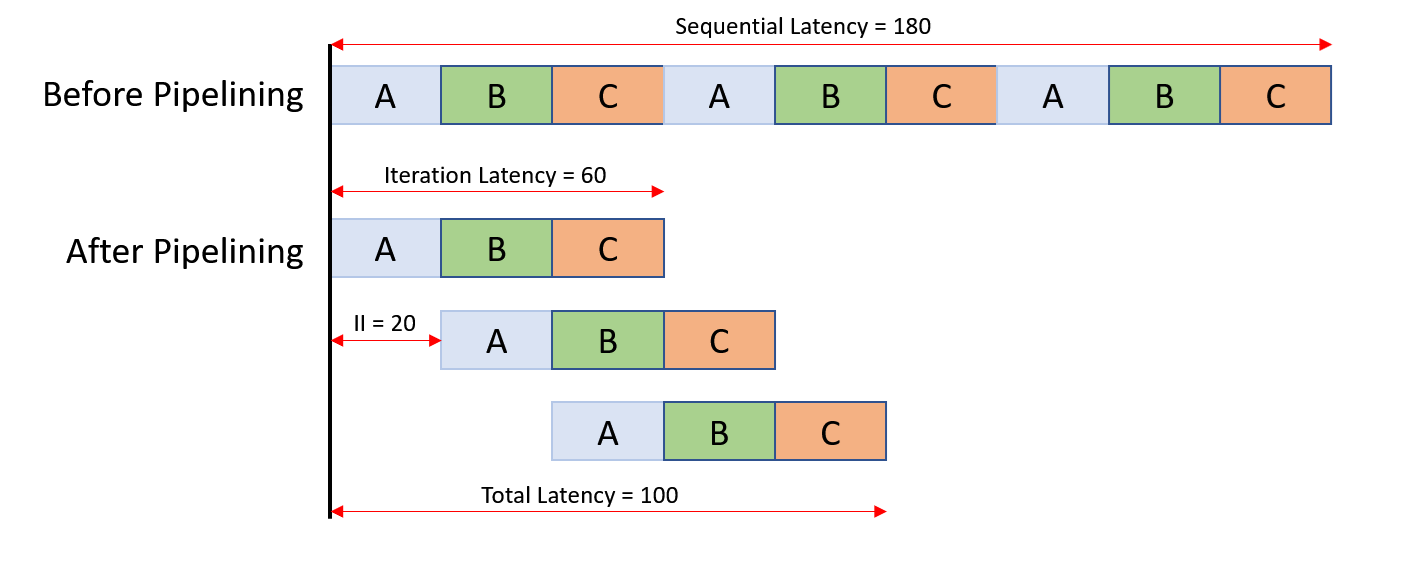
\includegraphics[width=.8\textwidth]{pipelining}
	\caption{Pipelining example.}
	\label{fig:pipeline}
\end{figure}

\subsubsection{Loop unrolling}
The logic of a rolled loop allows the execution of one iteration at a time: if
the loop iterates $N$ times and each iteration has a latency $L_{it}$, the
total loop latency is equal to ${L_{loop, rolled} := N \cdot L_{it}}$.

The loop unrolling technique instantiates the logic for executing $f$ iterations
at a time (where $f$ is the unrolling factor).
If there are no dependencies between different iterations, the latency of the
unrolled loop is: ${L_{loop, unrolled}(f) := \frac{N}{f} \cdot L_{it}}$.

\bigskip
Loop unrolling can improve both latency and throughput, but it is expensive in
terms of resource usage, since they are multiplied by $f$.

\begin{figure}[!htb]
	\centering
	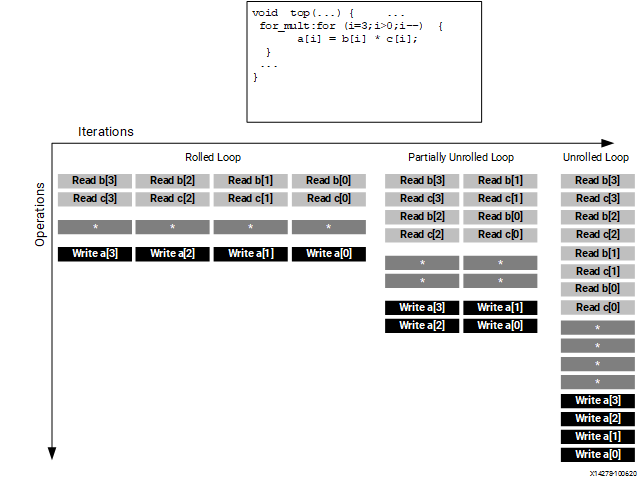
\includegraphics[width=.8\textwidth]{unroll}
	\caption{Loop unrolling example.}
\end{figure}

\subsubsection{Memory optimizations}
\begin{itemize}
	\item \underline{On-chip memory:}
		\begin{itemize}
			\item \textbf{Array partitioning}: given a partitioning
				factor $f$, an array is split into $f$
				portions, each one mapped to a dedicated memory
				element.

				This allows multiple concurrent accesses to the
				same array, at the cost of higher memory
				elements usage.

				Figure~\ref{fig:array_partitioning} shows
				different partitioning modes.
				\begin{figure}[!htb]
					\centering
					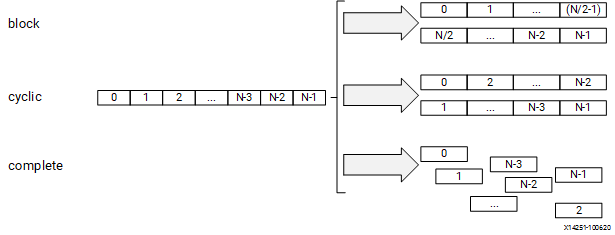
\includegraphics[width=.8\textwidth]{
						array_partitioning}
					\caption{Array partitioning examples.}
					\label{fig:array_partitioning}
				\end{figure}
		\end{itemize}
	\item \underline{Off-chip memory}:
		\begin{itemize}
			\item \textbf{Interface widening}: multiple data
				elements are packed into a single bigger word,
				to perform multiple accesses at the same time.
			\item \textbf{Burst accesses}: multiple memory accesses
				are aggregated into \ac{axi} bursts to reduce
				overall latency and improving throughput.
				\begin{figure}[!htb]
					\centering
					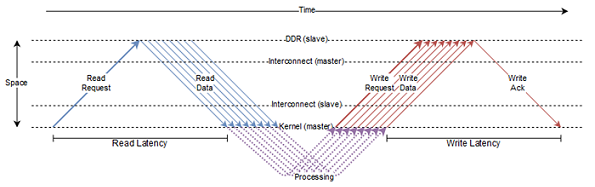
\includegraphics[width=.9\textwidth]{
						burst}
					\caption{Burst read and write example.}
				\end{figure}
		\end{itemize}
\end{itemize}

\chapter{Motivation}
\ac{hls} tools are currently unable to automatically exploit the memory
hierarchy present on \acp{fpga}: the only way to take advantage of
them is the manual management in a \emph{scratchpad}-like manner, which
requires additional design and verification efforts.

The proposed solution \textbf{automates the low-level memory management}
through a cache module for \ac{hls}, which works as an interface with the
off-chip \ac{dram} (accessible through an \ac{axi} bus) and stores its data to
on-chip \acp{bram} and registers.

\bigskip
The proposed cache module has the \textbf{dual purpose} of:
\begin{itemize}
	\item \emph{Reducing the number of \ac{dram} accesses}: misses only
		needs to access \ac{dram}.
	\item \emph{Optimizing \ac{dram} accesses}: lines are accessed in
		bursts through a widened memory interface.
\end{itemize}

\acp{fpga} provide multiple \ac{dram} ports and \ac{hls} can assign each array
to a different port: this allows implementing \textbf{array-specific} caches,
which in general can be easily tuned to reach high hit ratios, since access
patterns to a single array are usually regular and there is no interference
between accesses to different arrays.

\bigskip
A special attention has been put on \textbf{user-friendliness}:
\begin{itemize}
	\item \emph{Configurability}: cache characteristics can be set through
		parameters.
	\item \emph{Integrability}: cache can be inserted into existing designs
		without requiring many changes.
	\item \emph{Observability}: critical cache data (e.g.\ hit ratio) can
		be profiled during \ac{sw} simulation for easing the cache
		parameters tuning.
\end{itemize}

\section{Ma's cache}
Liang Ma et al.\ proposed a \texttt{C++} cache implementation~\cite{liang}
compatible with \emph{Vivado\texttrademark~HLS~2016.2}.

It is an array-specific cache module in the form of different \texttt{C++}
classes: each of them implements an access type (read only/write only and read
write) and a mapping policy (direct mapped and set associative).

To improve the \emph{integrability} the \texttt{operator[]} has been overloaded
so that the cache object can be accessed in the same way as array variables,
minimizing the required changes to the code which integrates the cache.

\bigskip
This architecture is \textbf{inlined}: the cache logic is directly inserted in
the user algorithm logic.
This is the major limitation of this solution, since the additional logic
inserted in the algorithm may make it too complex and worsen the generated
circuit performance.

\section{Proposed solution}
The primary goal of this thesis work is to develop the \emph{Basic cache}, a
cache architecture which runs in a separate process with respect to the
application using it, trying to solve the main limitation of \emph{Ma's cache}:
the application logic cluttering due to the inlining.

This architecture has been then optimized in two dimensions:
\begin{itemize}
	\item \emph{Multi-levels cache}: a \ac{l1} cache are added to the cache
		hierarchy, with the objective of further reducing memory access
		latency.
	\item \emph{Multi-ports cache}: multiple cache access points are added
		to the cache, each one with a dedicated \ac{l1} cache, so that
		multiple requests can be served in parallel.
\end{itemize}

\chapter{Basic cache}
The \emph{Basic cache} is aimed at solving the main limitation of \emph{Ma's
cache}: application logic cluttering due to inlining.

\section{Architecture}
The fundamental idea behind the \emph{Basic cache} is that the cache logic is
inserted in a separate process with respect to the application logic accessing
it (Figure~\ref{fig:single_proc_basic_arch}): this isolation makes the cache
always perform in the same manner, independently of the algorithm accessing it,
while keeping the application logic as clean as possible, since application
only has to write requests to cache and read responses, instead of integrating
the whole cache logic.

\begin{figure}[!htb]
	\centering
	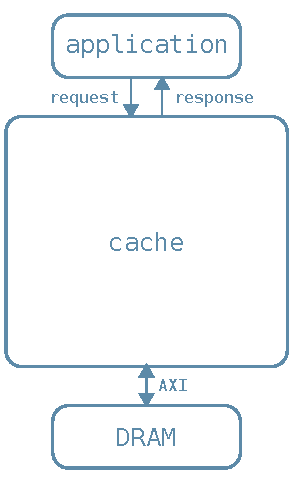
\includegraphics[width=.3\textwidth]{single_proc_basic_arch}
	\caption{\emph{Single-process Basic cache} architecture.}
	\label{fig:single_proc_basic_arch}
\end{figure}

\subsection{Functionality}
If application $A$ needs to access the array associated with the cache $C$:
\begin{enumerate}
	\item $A$ sends the access request to $C$: operation (i.e.\ read or
		write), address and (in case of write access) data.
	\item $C$ receives the request and checks if the requested address
		causes a miss.
	\item (in case of miss) $C$ prepares its \ac{bram} memory for fulfilling
		the requested access:
		\begin{itemize}
			\item (if needed) writes back to \ac{dram} the \ac{bram}
				line to be replaced.
			\item reads from \ac{dram} the requested line and store
				it to \ac{bram}.
		\end{itemize}
	\item $C$ performs the requested access to \ac{bram} and (in case of
		read request) sends requested data to $A$.
\end{enumerate}

\subsection{Characteristics}
The \emph{Basic cache} is compliant with the set associative mapping policy and
the write-back consistency policy.
It is configurable in terms of:
\begin{itemize}
	\item Word type and number of words per line.
	\item Number of sets and ways (therefore, it is possible to obtain a
		fully associative policy by setting the number of sets to 1 or
		a direct mapped policy by setting the number of ways to 1).
	\item Replacement policy (\acl{lru} or \acl{fifo}).
\end{itemize}

\subsection{Single-process Basic cache}
The \emph{Single-process Basic cache} is composed of a single pipelined process
which performs all the cache functionalities.

This process can be pipelined with an \ac{ii} equal to 1 when:
\begin{itemize}
	\item Memory accesses are Read-Only.
	\item A cache line can fit a single \ac{axi} transaction (i.e.\ line is
		not bigger than the maximum \ac{axi} interface width: 512 or
		1024 bits typically, depending on the specific device).
\end{itemize}

Write accesses generate some dependencies on the \ac{axi} interface, while large
cache lines require multiple \ac{axi} transactions: both of them cause an
increase of the cache process \ac{ii}, reducing cache performance.

\subsection{Multi-processes Basic cache}
The \emph{Multi-processes Basic cache} splits cache into two processes
(Figure~\ref{fig:multi_proc_basic_arch}):
\begin{itemize}
	\item \emph{Core} process: manages communication with application and
		keeps cache data structures up to date.
	\item \emph{Memory interface} process: deals with the \ac{axi}
		interface.
\end{itemize}

This architecture is aimed at solving the performance limitations of the
\emph{Single-process Basic cache}: it manages to pipeline the \emph{core}
process with an \ac{ii} equal to 1, even in case of write-only accesses or long
lines, since the \ac{axi} interfacing resides in the separate \emph{memory
interface} process.

The latency of the response to a hitting request depends on the \emph{core}
process only, therefore with this solution the best performance is achieved in
case of write-only caches too.

\bigskip
In the case of caches which are accessed both in read and in write mode, it has
not been possible to achieve an \ac{ii} of 1, due to dependencies on the cache
memory.
Given that a read-write cache implies at least one read access and one write
access, 

\begin{figure}[!htb]
	\centering
	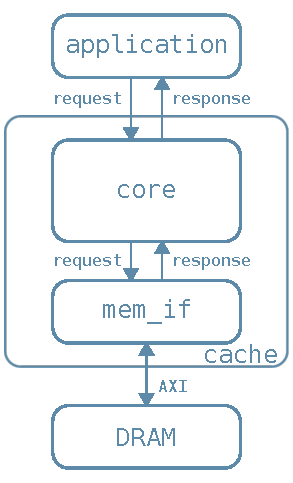
\includegraphics[width=.3\textwidth]{multi_proc_basic_arch}
	\caption{\emph{Multi-processes Basic cache} architecture.}
	\label{fig:multi_proc_basic_arch}
\end{figure}

\section{Implementation}\label{sec:basic_impl}
The \emph{Basic cache} is implemented in the form of a
\texttt{C++14}~\cite{cpp14} class, compatible with
\emph{Vitis\texttrademark~HLS~2021.1}.
All the configurable parameters are set through class template arguments.

The cache class is logically split into two parts:
\begin{itemize}
	\item \emph{Internals}: cache functionalities.
	\item \emph{Interface}: \acsp{api} for managing requests and responses
		from application side.
\end{itemize}

\emph{Internals} and \emph{Interface} communicate with each other through a
\emph{Port} (Table~\ref{tab:port}), in a \emph{Master/Slave} fashion:
\begin{itemize}
	\item \emph{Interface} sends to \emph{Internals} a \emph{request}
		(operation, address and write data).
	\item \emph{Internals} sends to \emph{Interface} a \emph{response}
		(read data), after executing the requested operation.
\end{itemize}

\begin{table}[!htb]
	\begin{center}
		\begin{tabular}{ccc}
			\hline
			\rowcolor{gray!50}
			\textbf{Content} & \textbf{Description} &
			\textbf{Direction} \\
			\hline
			Operation & Read/Write &
			\emph{Internals} $\rightarrow$ \emph{Interface} \\
			\rowcolor{gray!25}
			Address & Index to be accessed &
			\emph{Internals} $\rightarrow$ \emph{Interface} \\
			Write data & Data to be written to memory &
			\emph{Internals} $\rightarrow$ \emph{Interface} \\
			\rowcolor{gray!25}
			Read data & Data read from memory &
			\emph{Internals} $\leftarrow$ \emph{Interface} \\
			\hline
		\end{tabular}
	\end{center}
	\caption{Data exchanged through \emph{Port}.}
	\label{tab:port}
\end{table}

\paragraph{Process modeling}
\ac{hls} is intended for synthesizing sequential \acl{sw} code, therefore it has
been necessary to develop a novel technique for modeling multiprocess designs.

The proposed model follows the \emph{Master/Slave} paradigm:
\begin{enumerate}
	\item \emph{Master} sends a request to \emph{Slave}.
	\item \emph{Slave} executes the requested operation and optionally sends
		a response to \emph{Master}.
\end{enumerate}

\emph{Slave} must be modeled as an infinite loop which waits for requests from
\emph{Master} before executing its functionality, while \emph{Master} can be
modeled as standard sequential code (or it can be in turn a \emph{Slave} of
another \emph{Master}).

The parallelism between \emph{Master} and \emph{Slave} is modeled differently
depending on the compilation target:
\begin{itemize}
	\item \emph{\ac{sw} simulation}: each process is mapped to a
		\texttt{std::thread}.
	\item \emph{\ac{hw} synthesis}: each process is a dataflow function, in
		a dataflow region with the \texttt{disable\_start\_propagation}
		option disabled (which allow each function to run in parallel,
		without waiting for the completion of previous ones).
\end{itemize}
The distinction between simulation and synthesis code can be performed through
the ``\texttt{\#ifdef \_\_SYNTHESIS\_\_}'' preprocessor directive.

The communication between the two processes is performed through a \emph{port},
which contains data flowing from \emph{Master} to \emph{Slave} (request) and
from \emph{Slave} to \emph{Master} (response).
Request and response are mapped to one or more \acp{fifo} which are written
from the transmitter and read from the receiver.
\texttt{hls::stream} class by \emph{Vitis\texttrademark~HLS} can be used as
\ac{fifo} implementation.

\subsection{Internals}\label{subsec:basic_impl_internals}
The \emph{Internals} implementation differs between the \emph{Single-process}
and the \emph{Multi-processes} implementations:
\begin{itemize}
	\item \emph{Single-process Basic cache}: single process which
		implements all the cache functionalities.
	\item \emph{Multi-processes Basic cache}:
		\begin{itemize}
			\item \emph{Core} process: same as \emph{Single-process
				Basic cache} process, but it does not
				directly access the \ac{axi} bus: it issues
				requests to the \emph{memory interface} process
				through \acp{fifo}.
			\item \emph{Memory interface} process: it accesses the
				\ac{axi} bus as requested by the \emph{core}
				process.
		\end{itemize}
\end{itemize}

\emph{Single-process Basic cache}, with respect to the \emph{Multi-processes}
one, requires lower resource usage and better performance, when it is possible
to schedule its process with an \ac{ii} equal to 1 (read-only accesses with
line not larger than the maximum \ac{axi} interface bitwidth): therefore it is
automatically instantiated whenever it is convenient.

\subsubsection{Dataflow checking}
Alternatively executing the \emph{Multi-processes} or the \emph{Single-process}
code with traditional \texttt{if} statements would generate errors during the
synthesis, particularly in the \emph{Dataflow check} step (which checks if each
\texttt{hls::stream} has a single reader and a single writer): the compiler
builds both branches of the \texttt{if} statements, independently of the fact
that one of them is never executed.

\bigskip
The problem has been solved through a wrapper class, which conditionally
includes a \texttt{hls::stream} object, exploiting the template specialization
mechanism.

\subsubsection{Arrays partitioning}
Cache memory (which stores the actual data) must be accessed one line per clock
cycle: it is mapped to a \ac{bram} array cyclically partitioned with a factor
equal to the number of lines.

Helper data (e.g.\ \texttt{tag}, \texttt{valid}, \texttt{dirty}\ldots) is stored
to completely partitioned arrays, mapped to registers, in order to avoid
dependencies as much as possible and get the best performance.

\subsubsection{\ac{axi} optimizations}
To exploit the \emph{Vitis\texttrademark~HLS} support to automatic port
widening and burst accesses to \ac{axi} interface, every access to external
\ac{dram} accesses a whole cache line.
The accessed addresses \acp{lsb} are explicitly set to 0 so that synthesizer
can infer that they are aligned to the line size.

If the cache line is at most equal to the maximum \ac{axi} interface width, it
is accessed in a single request, otherwise it is accessed in multiple burst
requests.

\subsubsection{\acl{raw} dependencies}
In case of read-write caches, the \emph{Core} process \ac{ii} increases to 3
due to \ac{raw} dependencies on the cache \ac{bram}.

To mitigate this issue the \emph{\ac{raw} cache} has been developed: it is a
single-line cache which provides the functions:
\begin{itemize}
	\item \texttt{get\_line}: in case of hit, read the \emph{\ac{raw}
		cache} line; in case of miss, read the cache line.
	\item \texttt{set\_line}: write both the \emph{\ac{raw} cache} line and
		the cache line.
\end{itemize}

Cache memory is always accessed through the \emph{\ac{raw} cache} and the
\texttt{set\_line} function is called once per iteration at most: if a cache
line has been written, it is impossible that it is read in the next iteration,
since the \ac{raw} cache would hit and return its line. This allows to falsify
the \ac{raw} dependency with distance 1 on the cache memory (by setting to
\texttt{false} the \ac{raw} inter-iteration dependencies and to \texttt{true}
the \ac{raw} inter-iteration dependencies with distance 1).

\bigskip
This solution allows to schedule the cache process with an \ac{ii} equal to 2.
The \emph{\ac{raw} cache} could be extended to a fully-associative cache
complying with the \ac{fifo} replacement policy, allowing to falsify the
\ac{raw} dependency with distance 2 and achieving an \ac{ii} of 1.

\bigskip
A read-write cache implies that it is accessed at least two times per iteration
(once in read mode, once in write mode), therefore, due to the issues discussed
in Subsection~\ref{subsec:basic_impl_if} it is not possible to fully exploit the
cache pipelining.
In this case the cache \ac{ii} does not have a relevant impact on effective
performance: \emph{\ac{raw} cache} could not provide real advantages and it has
not been included in the final design, to keep it simpler.

\subsection{Interface}\label{subsec:basic_impl_if}
\emph{Interface} provides \acsp{api} for managing requests and responses between
application and cache:
\begin{itemize}
	\item \texttt{get}: send a read request and read the response.
	\item \texttt{set}: send a write request.
\end{itemize}
To improve user-friendliness, similarly to \emph{Ma's cache}, the
\texttt{operator[]} has been overloaded so that a cache object can be used as a
traditional array (e.g.\ \texttt{val~=~cache[i]} calls
\texttt{val~=~cache.get(i)} and \texttt{cache[i]~=~val} calls
\texttt{cache.set(i,~val)}).

\subsubsection{Deadlock prevention}
The \ac{hls} scheduler is not able to infer the dependency between the request
writing ($W$) and the response reading ($R$) in the \texttt{get} function
(i.e.\ it is not aware that first the request has to be written, then it is
necessary to wait for the cache latency and finally the response has to be
read).

For that reason the scheduler optimizes the logic by inserting both $W$ and $R$
into the same pipeline stage.
This leads to a deadlock: $R$ is blocked since it reads from an empty \ac{fifo}
(it cannot contain the response yet) and it blocks the whole stage, including
$W$, making $R$ wait for the response to a request which cannot be sent.

The deadlock has been fixed by inserting a clock operation between $W$ and $R$
(calling \texttt{ap\_wait}), which forces $W$ and $R$ to separate pipeline
stages.

\subsubsection{Cache pipeline exploiting}
At the steady state, in case of hit, the cache can process one request per
cycle, thanks to its optimal pipelining (i.e.\ \ac{ii} equal to 1).

\ac{hls} is not aware of the dependency and latency between request writing
($W$) and response read ($R$), so it schedules $R$ just after $W$
(Figure~\ref{subfig:actual_sched_static}): at runtime $R_i$, which should be
executed in the cycle following $W_i$, stalls, since the cache response has a
latency (and $W_{i+1}$ stalls too, by consequence).

$W_{i+1}$ is executed after waiting for the full latency of the cache
(Figure~\ref{subfig:actual_sched_run}) and the final result is that cache never
receives multiple requests in consecutive cycles, it never reaches the steady
state and its throughput is the same as if it were not pipelined.

\begin{figure}[!htb]
	\centering
	\begin{subfigure}[b]{.3\textwidth}
		\centering
		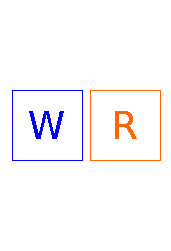
\includegraphics[height=2.5cm]{actual_schedule_static}
		\caption{Static schedule.}
		\label{subfig:actual_sched_static}
	\end{subfigure}
	\hfill
	\begin{subfigure}[b]{.68\textwidth}
		\centering
		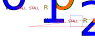
\includegraphics[height=2.5cm]{actual_schedule_run}
		\caption{Runtime.}
		\label{subfig:actual_sched_run}
	\end{subfigure}
	\caption{Stalling schedule of request writing and response reading.}
	\label{fig:actual_sched}
\end{figure}

\bigskip
To mitigate this issue the \texttt{ap\_wait} between request write and response
read has been replaced with \texttt{ap\_wait\_n(LATENCY)}, where
\texttt{LATENCY} is an integer value set through a template parameter.
This forces the scheduler to insert \texttt{LATENCY} clock cycles between $W$
and $R$ (Figure~\ref{subfig:desired_sched_static}), so that at runtime stalls
are avoided (in case of hit) and one request per cycle is sent to cache
(Figure~\ref{subfig:desired_sched_run}).

\begin{figure}[!htb]
	\centering
	\begin{subfigure}[b]{.3\textwidth}
		\centering
		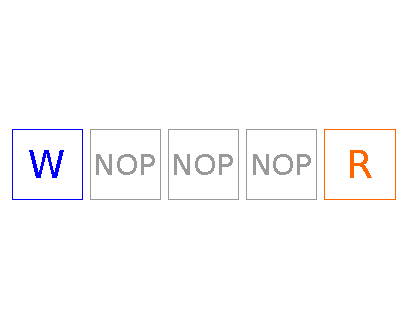
\includegraphics[height=3cm]{desired_schedule_static}
		\caption{Static schedule.}
		\label{subfig:desired_sched_static}
	\end{subfigure}
	\hfill
	\begin{subfigure}[b]{.68\textwidth}
		\centering
		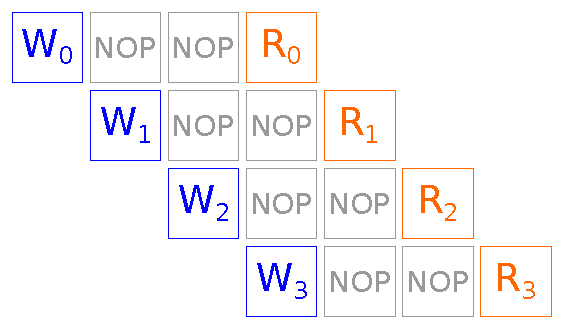
\includegraphics[height=3cm]{desired_schedule_run}
		\caption{Runtime.}
		\label{subfig:desired_sched_run}
	\end{subfigure}
	\caption{Optimal schedule of request writing and response reading.}
	\label{fig:desired_sched}
\end{figure}

\texttt{LATENCY} is not set to a constant because its optimal value highly
depends on memory access pattern and cache configuration, and can be determined
by means of design exploration.

This is a partial solution: the \texttt{ap\_wait} forces all the subsequent
operations to wait: when there are multiple calls to \texttt{get} per
iteration (e.g.\ $A$ and $B$), $W_B$ has to wait \texttt{LATENCY} cycles after
$W_A$ before being scheduled (Figure~\ref{subfig:fixed_sched_issue}).
This situation makes the application loop \ac{ii} to increase, since it must
guarantee the order of accesses to \acp{fifo} (i.e.\ $W_{A, i+1}$ cannot be
executed before $W_{B, i}$).

\bigskip
To actually fix this problem (with the schedule shown in
Figure~\ref{subfig:fixed_sched_desired}), a mechanism for informing the
scheduler about dependencies and latency between specific operations is
probably needed, but this is not available in
\emph{Vitis\texttrademark~HLS~2021.1}.

\begin{figure}[!htb]
	\centering
	\begin{subfigure}[b]{.4\textwidth}
		\centering
		
\includegraphics[height=1.4cm]{fixed_schedule_issue}
		\caption{Achieved static schedule.}
		\label{subfig:fixed_sched_issue}
	\end{subfigure}
	\hfill
	\begin{subfigure}[b]{.4\textwidth}
		\centering
		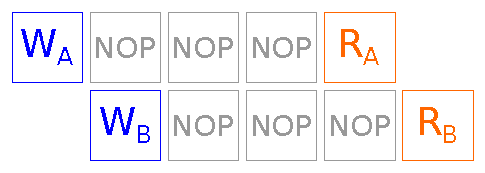
\includegraphics[height=1.4cm]{fixed_schedule_desired}
		\caption{Optimal static schedule.}
		\label{subfig:fixed_sched_desired}
	\end{subfigure}
	\caption{Static schedules in case of multiple accesses per iteration.}
	\label{fig:fixed_sched_issue}
\end{figure}

\chapter{Multi-levels cache}
The \emph{Multi-levels cache} is aimed at improving performance by making the
memory hierarchy deeper, adding a faster \ac{l1} cache memory on top of it.
This alternative approach has been proposed to overcome the difficulties, to
fully exploit the optimal pipeline of the \emph{Basic cache}, due to the
scheduler unawareness about the latency between request writing and response
reading (as explained in Section~\ref{sec:basic_impl}).

\section{Architecture}
The \emph{Multi-levels cache} introduces a \ac{l1} cache inlined in the
application logic (Figure~\ref{fig:l1_arch}): the scheduler exactly knows the
latency of each \ac{l1} cache operation and can build an application pipeline
which stalls in case of \ac{l1} miss only.

In order not to fall into the same cluttering issues of \emph{Ma's cache}, the
\ac{l1} cache is kept as simple as possible:
\begin{itemize}
	\item Mapping policy: direct-mapped.
	\item Consistency policy: write-through.
\end{itemize}

The write-through consistency policy discards any advantage for write accesses,
but given that simplicity is a priority and read accesses are usually more
frequent than writes, and they suffer the most from the scheduling issues which
lead to the introduction of the \ac{l1} cache, this has been considered the
best trade-off.

\begin{figure}[!htb]
	\centering
	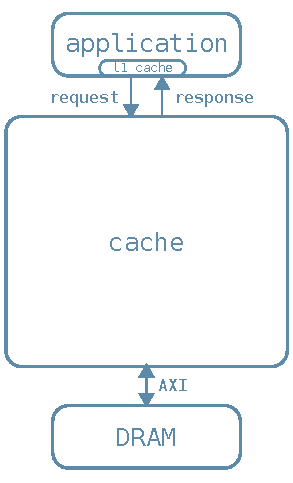
\includegraphics[width=.3\textwidth]{l1_arch}
	\caption{\emph{Multi-levels cache} architecture.}
	\label{fig:l1_arch}
\end{figure}

\section{Implementation}
The \emph{Multi-level cache} has been implemented adding the \ac{l1} cache to
the \emph{Basic cache}.
It is possible to configure the number of \ac{l1} cache lines through the
\texttt{L1\_CACHE\_LINES} template parameter.
When it is set to 0, the resulting architecture is equivalent to the \emph{Basic
cache}.

\subsection{Internals}
The only difference with respect to the \emph{Basic cache} implementation is
that the response to a read request does not send a single word, but a whole
cache line (therefore the data \ac{fifo} flowing from cache to application
has been widened accordingly).

\subsection{Interface}
The \ac{l1} cache is contained in the \emph{Interface}: the newly introduced
\texttt{get\_line} function receives an address $A$ in input and it returns the
line to which $A$ belongs.
In particular, it first checks if $A$ hits in the \ac{l1} cache: if so it reads
the data from the \ac{l1} cache, otherwise it issues the request to the \ac{l2}
cache.

\bigskip
It is still possible to use the same \emph{Basic cache} \acp{api}, which have
been updated to support the \ac{l1} cache:
\begin{itemize}
	\item \texttt{get}: it calls the \texttt{get\_line} function and then
		returns the requested word.
	\item \texttt{set}: it sets \ac{l1} cache line to dirty, if it hits, and
		it forwards the request to the \ac{l2} cache.
\end{itemize}

\chapter{Multi-ports cache}
The computational core of many algorithms consists in a loop, which \ac{hls} can
optimize with two techniques: \emph{Pipelining} and \emph{Unrolling}.

The \emph{Basic} and \emph{Multi-levels} caches are suitable for
\emph{Pipelining} since they complete one access per clock cycle, at the steady
state, in case of hit, however they are not suitable for \emph{Unrolling}, since
they do not support concurrent accesses.

\bigskip
The \emph{Multi-ports cache} has been specifically designed for adding support
to multiple \textbf{concurrent accesses} to the same cache memory, allowing to
efficiently \textbf{unroll} application loops.

\section{Architecture}
The \emph{Multi-ports cache} is characterized by multiple ports accessed in
parallel (Figure~\ref{fig:multi_ports_arch}).

Each port has dedicated logic for communicating with the shared \ac{l2} cache
and an independent \ac{l1} cache.

\bigskip
Multiple independent ports allow \textbf{removing dependencies} between
different accesses to the cache.
This brings the advantage of achieving better performance, making it possible
to schedule multiple requests at the same time, without increasing the
application loop \ac{ii}, but it also brings the disadvantage of not
guaranteeing the expected ordering between different accesses.
To guarantee the correct functionality the \emph{Multi-ports} architecture is
compatible with \textbf{read-only} accesses.

\begin{figure}[!htb]
	\centering
	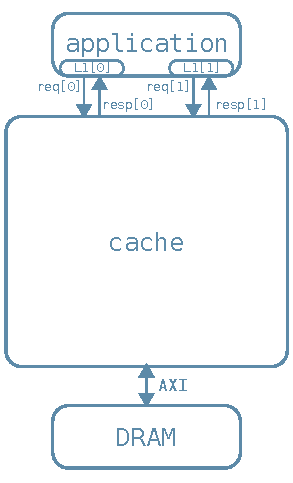
\includegraphics[width=.3\textwidth]{multi_ports_arch}
	\caption{\emph{Multi-ports cache} architecture.}
	\label{fig:multi_ports_arch}
\end{figure}

\section{Implementation}
The \emph{Multi-ports cache} has been implemented extending the
\emph{Multi-levels cache}.

It is possible to configure the number of ports through the \texttt{PORTS}
template parameter.
When it is set to 1, the resulting architecture is equivalent to the
\emph{Multi-levels cache}.

\subsection{Internals}
To avoid dependencies issues, whenever \texttt{PORTS} is greater than 1, the
\emph{Multi-process} \emph{Internals} architecture is generated.

\bigskip
The \emph{Core} process has been modified to serve requests coming from all the
ports by inserting an unrolled loop which iterates over all the ports. \ac{hls}
guarantees all the dependencies on cache data structures, and the resulting
\ac{ii} of the \emph{Core} process is equal to \texttt{PORTS}.

\subsection{Interface}
\acp{fifo} between \emph{Core} and application and \ac{l1} cache have been
replaced with arrays of \acp{fifo} and \ac{l1} caches, completely partitioned,
so that they are independent.

Each call to \texttt{get\_line} (which is in turn called by \texttt{get}) is
automatically associated with a specific port by means of a member variable
holding the port index and is updated after each access.

\subsubsection{\acp{fifo} accesses scheduling}
Ideally the request write ($W$) and the response read ($R$) should be scheduled
in parallel in the same cycle (Figure~\ref{subfig:multiport_des_sched}).
Due to the scheduler limitations (described in
Subsection~\ref{sec:basic_impl}) it is not possible to achieve such a
schedule, since there is a forced clock cycle between $W$ and $R$, which delays
all the subsequent operations.

The resulting schedule (Figure~\ref{subfig:multiport_actual_sched}) is almost
equivalent to the one achieved with the \emph{Basic cache} in case of multiple
accesses per iteration (Figure~\ref{subfig:fixed_sched_issue}), with the
difference that request and response \acp{fifo} are distinct, since they belong
to separate ports, therefore the scheduler does not have to ensure dependencies
between subsequent reads and writes and application loop \ac{ii} does not
increase.

At the steady state, in case of hit, one $W$ and $R$ are executed per cycle,
allowing to fully exploit the \ac{l2} cache pipeline.

\begin{figure}[!htb]
	\centering
	\begin{subfigure}[b]{.4\textwidth}
		\centering
		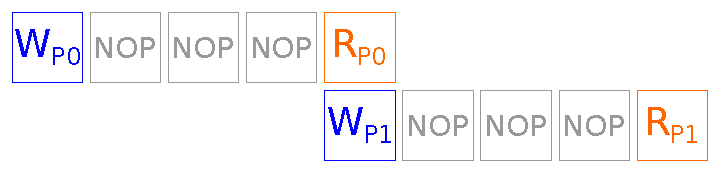
\includegraphics[height=1.4cm]{multiport_actual_sched}
		\caption{Achieved static schedule.}
		\label{subfig:multiport_actual_sched}
	\end{subfigure}
	\hfill
	\begin{subfigure}[b]{.4\textwidth}
		\centering
		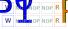
\includegraphics[height=1.4cm]{multiport_des_sched}
		\caption{Parallel static schedule.}
		\label{subfig:multiport_des_sched}
	\end{subfigure}
	\caption{Static schedules in case of 2-ports cache.}
	\label{fig:multiport_sched}
\end{figure}

\section{Limitations}
In some particular situations (e.g.\ when cache is explicitly accessed multiple
times per iteration) the simulation of the generated circuit enters a deadlock.
The source of this problem can be probably found in the port indexing and to be
fixed may require more control over the operations scheduling, which is not
provided by \emph{Vitis\texttrademark~HLS 2021.1}.

\chapter{Results}
The proposed cache architecture has been embedded in multiple \emph{Vitis~HLS}
kernels implementing different algorithms, to evaluate both the performance gain
and the resource usage of different cache configurations.

Each algorithm has been selected for its memory intensiveness and for its
specific memory access patterns.

\section{Simulation environment}
Kernels have been synthesized by the C Synthesis in
\emph{Vitis\texttrademark~HLS~2021.1}, targeting the
\texttt{xcvu9p-flgb2104-2-e} part, running at a clock frequency of $250 MHz$.

\emph{Vitis\texttrademark~2021.1} provides two main kind of simulation:
\begin{itemize}
	\item \acl{hw} Emulation: accurate, but slow.
	\item C/\acs{rtl} Co-Simulation: fast, but not very accurate
		(especially for what concerns the \ac{axi} interface model).
\end{itemize}

\ac{hw} Emulation has been used for determining the delay of the \ac{axi}
interface (which is around 4 clock cycles). 
The \ac{axi} latency has been accordingly set to 3, so that the synthesizer can
better optimize the circuit and Co-Simulation results match \ac{hw} emulation as
much as possible.

\begin{table}[!htb]
	\begin{center}
		\begin{tabular}{ll}
			\hline
			\rowcolor{gray!25}
			\textbf{Synthesizer} & C Synthesis in
			\emph{Vitis\texttrademark~HLS~2021.1} \\
			\textbf{Simulator} & C/RTL Co-Simulation in
			\emph{Vitis\texttrademark~HLS~2021.1} \\
			\rowcolor{gray!25}
			\textbf{Flow target} & \texttt{vitis} \\
			\textbf{Part codename} & \texttt{xcvu9p-flgb2104-2-e} \\
			\rowcolor{gray!25}
			\textbf{Clock period} & $4 ns$ \\
			\textbf{\ac{axi} latency} & 3 \\
			\hline
		\end{tabular}
	\end{center}
	\caption{Simulation environment configuration.}
	\label{tab:sim_config}
\end{table}

\subsection{Reference memory models}
The results have been compared with the output of synthesis and simulation of
same algorithms implemented with different data access mechanisms: \emph{global
memory} (performance lower bound) and \emph{local memory} (performance higher
bound).

\subsubsection{Global memory}
The algorithms access data directly from external \ac{dram} through \ac{axi}
interface: this is the straightforward but slowest solution, therefore it
determines the performance lower bound.

\subsubsection{Local memory}
All the data required by algorithms is stored to local \acp{bram}: it determines
the performance higher bound, but it is unfeasible in general, due to the
limited amount of \acp{bram}.

With this solution the kernel:
\begin{enumerate}
	\item Moves all the input data from \ac{dram} to \acp{bram}.
	\item Performs all the computations accessing data to and from
		\acp{bram}. 
	\item Moves all the output data from \acp{bram} to \ac{dram}.
\end{enumerate}

The execution time of \ac{dram} accesses is not of interest, therefore it has
been subtracted from reported results.

\subsubsection{Ma's cache}
\emph{Ma's cache} was designed for \emph{Vivado\texttrademark~HLS~2016.2}:
with some minor changes it is possible to synthesize it with
\emph{Vitis~HLS~2021.1}, but it would need some more optimizations to achieve
the original performance in the new environment.

The results reported in Ma's paper \citetitle{liang} and PhD thesis
\citetitle{liangthesis} are not comparable with the ones obtained in
\emph{Vitis~HLS~2021.1}: the execution times of same algorithms with same
configurations (i.e.\ global and local memory) differ up to one order of
magnitude (most probably due to different \ac{axi} latency values), therefore
also cache execution times would not be reliable for making comparisons.

The lack of comparable results and the impossibility to generate new ones
prevented from directly comparing the proposed cache results with the Ma's
ones.

\clearpage

\subsection{Collected data}
The most relevant collected data concerns:
\begin{itemize}
	\item Performance: evaluated in terms of execution time (i.e.\ the time
		at which the simulation of the algorithm terminates).
	\item Resource usage: evaluated in terms of number of used \acp{bram},
		\acp{dsp}, \acp{lut} and \acp{ff}.
\end{itemize}

These values are approximate, since they come from C/\ac{rtl} Co-Simulation and
from the estimations performed by the C Synthesis, but in any case they can be
meaningful for identifying some trends.

\clearpage

\section{Matrix multiplication}
The standard row-by-column \emph{Matrix multiplication} algorithm
(Algorithm~\ref{alg:matmul}) includes two memory access patterns: by rows ($A$
and $C$) and by columns ($B$).

Each row of $A$ matrix is accessed $P$ times and then it is not accessed
anymore: the most convenient $A$ cache is composed of a single line which fits a
matrix row, which is filled each time a new row is accessed and it hits until
the next row is accessed.

Each column of $B$ matrix is accessed $P$ times: the $B$ cache, to get a hit
ratio greater than 0 needs to contain at least $M$ lines and comply with the
fully-associative mapping policy.
The results reported by Ma used a direct-mapped cache with $M$ lines each one
containing $P$ elements (so that it is as big as the $B$ matrix).

$C$ elements are accessed sequentially and only once: any single-line cache with
$n$ words per line would have a hit ratio of $\frac{n - 1}{n}$.

\bigskip
The implementation used during the tests applies both pipelining and unrolling
(with factor equal to the number of ports) to the innermost loop.

\begin{algorithm}
	\caption{\emph{Matrix multiplication} algorithm.}\label{alg:matmul}
	\begin{algorithmic}
		\Require $A \in \mathbb{R}^{N \times M},
		B \in \mathbb{R}^{M \times P}, C \in \mathbb{R}^{N \times P}$
		\Ensure $C = A \times B$
		\Procedure{Multiply}{$A, B, C$}
			\For{$i = 0, \dots, N - 1$}
				\For{$j = 0, \dots, P - 1$}
					\State $tmp \gets 0$
					\For{$k = 0, \dots, M - 1$}
						\State $tmp \gets tmp +
							A[i][k] \cdot B[k][j]$
					\EndFor
					\State $C[i][j] \gets tmp$
				\EndFor
			\EndFor
		\EndProcedure
	\end{algorithmic}
\end{algorithm}

\subsection{16x16 matrices}
In the case of \emph{Matrix multiplication 16x16}, matrices $A$, $B$ and $C$ are
sized $16 \times 16$ ($N = 16, M = 16, P = 16$).

This problem has been explored in two configurations: \emph{Single-level cache
configuration} (\ac{l2} caches only), and \emph{Multi-level cache
configuration} (\ac{l2} and \ac{l1} caches).

\subsubsection{Single-level cache configuration}
The cache sizes have been fixed with the values shown in
Table~\ref{tab:matmul_16_no_l1_config}. The \texttt{get} latency and the number
of ports have been determined through design space exploration.

\begin{table}[H]
	\begin{center}
		\begin{tabular}{cccccc}
			\hline
			\rowcolor{gray!50}
			\textbf{Matrix} &
			\textbf{Sets} & \textbf{Ways} & \textbf{Words per line} &
			\textbf{\ac{l1} lines} & \textbf{Hit ratio} \\
			\hline
			$A$ & 1 & 1 & 16 & 0 & 99.6 \% \\
			\rowcolor{gray!25}
			$B$ & 16 & 1 & 16 & 0 & 99.6 \% \\
			$C$ & 1 & 1 & 16 & 0 & 93.8 \% \\
			\hline
		\end{tabular}
	\end{center}
	\caption{Single-level cache configuration for \emph{Matrix
	multiplication 16x16}.}
	\label{tab:matmul_16_no_l1_config}
\end{table}

Figure~\ref{fig:matmul_16_no_l1_space} shows the execution time with respect to
the \texttt{get} latency, for different numbers of ports.

It is worth noting that the \texttt{get} latency has a big impact on effective
performance, especially in the single-port case (one order of magnitude).
This makes clear that the cache process itself can run at high speed and the
bottleneck is the scheduling of the \acp{fifo} accesses.

Increasing the number of ports can provide significant advantages when the
\texttt{get} latency is not optimal, because multi-port allow to schedule some
cache requests in consecutive clock cycles.

\begin{figure}[H]
	\centering
	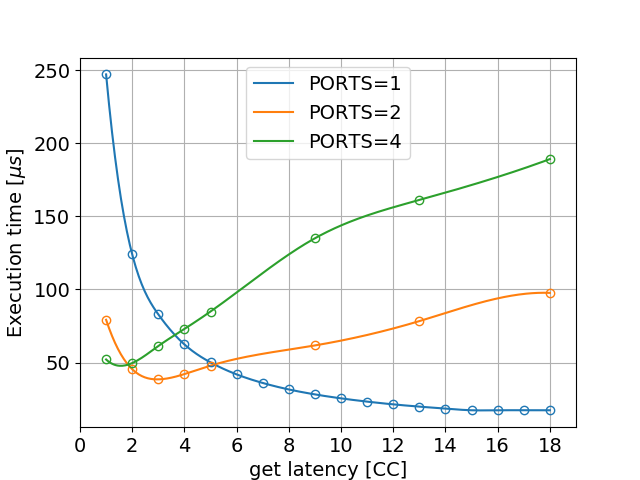
\includegraphics[width=.7\textwidth]{matmul_16_multiport_latency}
	\caption{Design space of \emph{Matrix multiplication 16x16}
	(single-level).}
	\label{fig:matmul_16_no_l1_space}
\end{figure}

The best performance is achieved by the single-port, since in this case the
caches \emph{core} process has an \ac{ii} of 1: with a \texttt{get} latency of
1 it is not possible to take full advantage of the \texttt{core} pipelining (as
explained in Subsection~\ref{subsec:basic_impl_internals}), therefore the
design keeps stalling even at the steady state
(Figure~\ref{subfig:matmul_wf_latency_1}: a new request is written every
multiple cycles) but the optimal \texttt{get} latency allows to fully exploit
the pipelining and at every cycle one request is written and a new response is
read (Figure~\ref{subfig:matmul_wf_latency_15}). 

\begin{figure}[H]
	\centering
	\begin{subfigure}[b]{.85\textwidth}
		\centering
		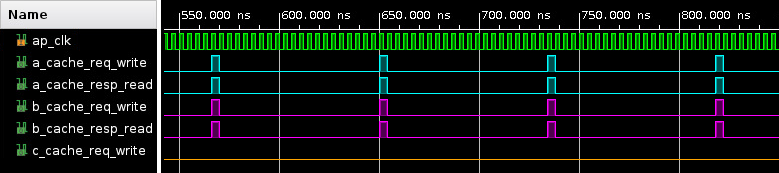
\includegraphics[width=\textwidth]{matmul_latency_1}
		\caption{Sub-optimal \texttt{get} latency of 1.}
		\label{subfig:matmul_wf_latency_1}
	\end{subfigure}
	\begin{subfigure}[b]{.85\textwidth}
		\centering
		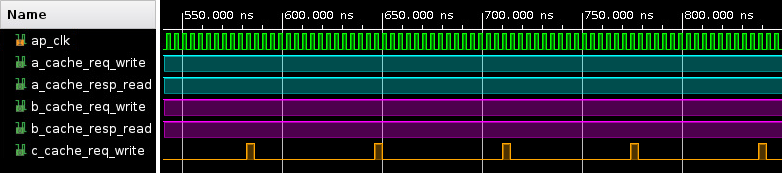
\includegraphics[width=\textwidth]{matmul_latency_15}
		\caption{Optimal \texttt{get} latency of 15.}
		\label{subfig:matmul_wf_latency_15}
	\end{subfigure}
	\caption{Request and response waveforms for \emph{Matrix multiplication
	16x16} single-level and single-port.}
	\label{fig:matmul_wf}
\end{figure}

Table~\ref{tab:matmul_16_no_l1_ports_report} reports the data for the
single-level cache configuration of different port numbers, each one set to its
optimal \texttt{get} latency value (15 for the 1-port, 3 for the 2-ports and 2
for the 4-ports).

It is not clear why the estimated required \acp{bram} in the 2-ports case is much
higher than the other cases.

\begin{table}[H]
	\begin{center}
		\begin{tabular}{cccc}
			\hline
			\rowcolor{gray!50}
			& \textbf{1-port} & \textbf{2-ports} & \textbf{4-ports} \\
			\hline
			\textbf{Execution time} [$ns$] & 17438 & 38570 & 49694 \\
			\rowcolor{gray!25}
			\textbf{\ac{bram}} & 90 & 165 & 90 \\
			\textbf{\acs{dsp}} & 3 & 6 & 12 \\
			\rowcolor{gray!25}
			\textbf{\acs{lut}} & 57653 & 87437 & 118434 \\
			\textbf{\acs{ff}} & 26597 & 37686 & 39352 \\
			\hline
		\end{tabular}
	\end{center}
	\caption{Performance and resource usage of \emph{Matrix multiplication
	16x16} (single-level).}
	\label{tab:matmul_16_no_l1_ports_report}
\end{table}

\subsubsection{Multi-levels cache configuration}
The cache sizes have been fixed with the values shown in
Table~\ref{tab:matmul_16_l1_config}.
The \texttt{get} latency and the number of ports have been determined through
design space exploration.

\begin{table}[H]
	\begin{center}
		\begin{tabular}{cccccc}
			\hline
			\rowcolor{gray!50}
			\textbf{Matrix} &
			\textbf{Sets} & \textbf{Ways} & \textbf{Words per line} &
			\textbf{\ac{l1} lines} & \textbf{Hit ratio} \\
			\hline
			$A$ & 1 & 1 & 16 & 1 & 99.6 \% \\
			\rowcolor{gray!25}
			$B$ & 1 & 1 & 16 & 16 & 99.6 \% \\
			$C$ & 1 & 1 & 16 & 0 & 93.8 \% \\
			\hline
		\end{tabular}
	\end{center}
	\caption{Multi-levels cache configuration for \emph{Matrix
	multiplication 16x16}.}
	\label{tab:matmul_16_l1_config}
\end{table}

From Figure~\ref{fig:matmul_16_l1_space} it is clear that the \texttt{get}
latency is not relevant is this case, since all the cache hits are on the
\ac{l1} cache.

Increasing the number of ports allows to significantly improve performance,
since the multiple \ac{l1} caches can run effectively in parallel, but the
higher is the number of ports, the lower is the hit ratio of \ac{l1} caches: 4
ports is the optimal configuration for what concerns performance.

\begin{figure}[H]
	\centering
	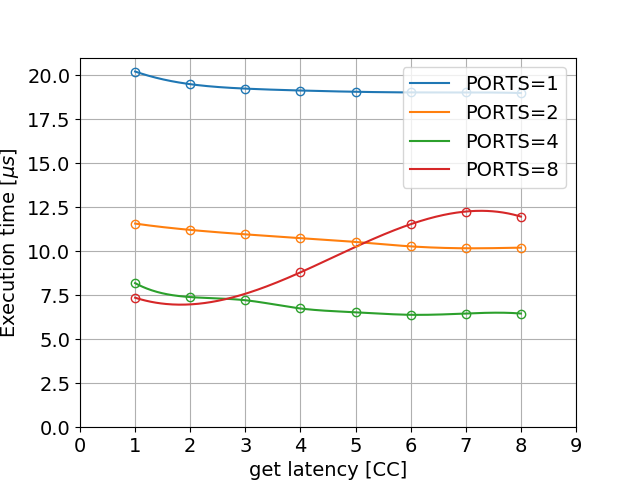
\includegraphics[width=.8\textwidth]{matmul_16_multiport_L1_latency}
	\caption{Design space of \emph{Matrix multiplication 16x16}
	(multi-levels).}
	\label{fig:matmul_16_l1_space}
\end{figure}

\begin{table}[H]
	\begin{center}
		\begin{tabular}{ccccc}
			\hline
			\rowcolor{gray!50}
			& \textbf{1-port} & \textbf{2-ports} & \textbf{4-ports}
			& \textbf{8-ports} \\
			\hline
			\textbf{Execution time} [$ns$] & 18986 & 10166 & 6458 &
			7358 \\
			\rowcolor{gray!25}
			\textbf{\ac{bram}} & 129 & 165 & 237 & 381 \\
			\textbf{\acs{dsp}} & 3 & 6 & 12 & 24 \\
			\rowcolor{gray!25}
			\textbf{\acs{lut}} & 58138 & 81779 & 118794 & 198678 \\
			\textbf{\acs{ff}} & 41961 & 101315 & 238374 & 581204 \\
			\hline
		\end{tabular}
	\end{center}
	\caption{Performance and resource usage of \emph{Matrix multiplication
	16x16} (multi-levels).}
	\label{tab:matmul_16_l1_ports_report}
\end{table}

\subsubsection{Summary}
Table~\ref{tab:matmul_16_report} reports most relevant figures about
performance and resource usage of \emph{Matrix multiplication 16x16}.

The Proposed cache data is referred to the most performant cases of the
single-level variant (with single port and \texttt{get} latency equal to 15)
and of the multi-levels variant (with 4 ports and \texttt{get} latency equal to
7).

The cost in terms of resource usage of the proposed cache is significant in
terms of resource usage, particularly the number of \acp{lut} and \acp{ff} is
one order of magnitude more for the single-level and single-port configuration
and two orders of magnitude for the multi-levels and multi-ports configuration,
with respect to global memory.
The single-level configuration allows reaching performance on par with the
local memory and the multi-level configuration is more than two times faster,
thanks to the unrolling.

\begin{table}[H]
	\begin{center}
		\begin{tabularx}{\textwidth}{CCCCC}
			\hline
			\rowcolor{gray!50}
			& \textbf{Global memory} & \textbf{Local memory} &
			\textbf{Proposed cache (single-level)} &
			\textbf{Proposed cache (multi-levels)} \\
			\hline
			\textbf{Execution time} [$ns$] & 30182 & 16916 & 17438
			& 6458 \\
			\rowcolor{gray!25}
			\textbf{\ac{bram}} & 34 & 90 & 90 & 237 \\
			\textbf{\acs{dsp}} & 3 & 3 & 3 & 12 \\
			\rowcolor{gray!25}
			\textbf{\acs{lut}} & 4421 & 26403 & 57653 &
			118794 \\
			\textbf{\acs{ff}} & 4736 & 8829 & 26597 & 238374 \\
			\hline
		\end{tabularx}
	\end{center}
	\caption{Performance and resource usage of \emph{Matrix multiplication
	16x16}.}
	\label{tab:matmul_16_report}
\end{table}

\clearpage

\subsection{32x32 matrices}
To check whether the results scale with the problem size, in the case of
\emph{Matrix multiplication 32x32}, matrices $A$, $B$ and $C$ have been sized
$32 \times 32$ ($N = 32, M = 32, P = 32$).

\subsubsection{Single-level cache configuration}
The cache sizes have been fixed with the values shown in
Table~\ref{tab:matmul_32_no_l1_config}. The \texttt{get} latency and the number
of ports have been determined through design space exploration.

\begin{table}[H]
	\begin{center}
		\begin{tabular}{cccccc}
			\hline
			\rowcolor{gray!50}
			\textbf{Matrix} & \textbf{Sets} & \textbf{Ways} &
			\textbf{Words per line} & \textbf{\ac{l1} lines} &
			\textbf{Hit ratio} \\
			\hline
			$A$ & 1 & 1 & 32 & 0 & 99.9 \\
			\rowcolor{gray!25}
			$B$ & 32 & 1 & 32 & 0 & 99.9 \\
			$C$ & 1 & 1 & 32 & 0 & 96.9 \\
			\hline
		\end{tabular}
	\end{center}
	\caption{Single-level cache configuration for \emph{Matrix
	multiplication 32x32}.}
	\label{tab:matmul_32_no_l1_config}
\end{table}

From Figure~\ref{fig:matmul_32_no_l1_space} it is possible to infer that the
shapes of the Execution time - \texttt{get} latency plot of \emph{Matrix
multiplication 32x32} are equivalent to the ones obtained in the \emph{16x16}
case.

\begin{figure}[H]
	\centering
	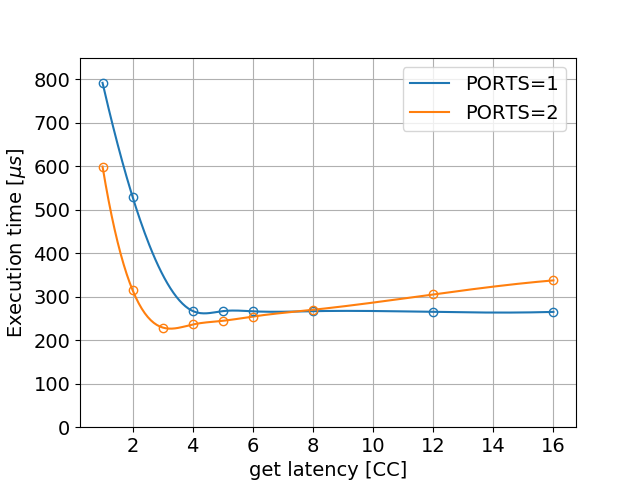
\includegraphics[width=.8\textwidth]{matmul_32_multiport_no_L1_latency}
	\caption{Design space of \emph{Matrix multiplication 32x32}
	(single-level).}
	\label{fig:matmul_32_no_l1_space}
\end{figure}

Results reported by Table~\ref{tab:matmul_32_no_l1_report} have been obtained
by setting the \texttt{get} latency to value which provided the best performance
(12 for the single-port cache and 3 for the dual-port cache).
The performance gain obtained by doubling the number of ports is not very
significant.

\begin{table}[H]
	\begin{center}
		\begin{tabular}{ccccc}
			\hline
			\rowcolor{gray!50}
			& \textbf{1-port} & \textbf{2-ports} \\
			\hline
			\textbf{Execution time} [$ns$] & 265226 & 229190 \\
			\rowcolor{gray!25}
			\textbf{\ac{bram}} & 90 & 90 \\
			\textbf{\acs{dsp}} & 3 & 6 \\
			\rowcolor{gray!25}
			\textbf{\acs{lut}} & 126411 & 175727 \\
			\textbf{\acs{ff}} & 39871 & 47648 \\
			\hline
		\end{tabular}
	\end{center}
	\caption{Performance and resource usage of \emph{Matrix multiplication
	32x32} (single-level).}
	\label{tab:matmul_32_no_l1_report}
\end{table}

\subsubsection{Multi-levels cache configuration}
The cache sizes have been fixed with the values shown in
Table~\ref{tab:matmul_32_l1_config}. Since most of the read accesses are
performed to \ac{l1} caches (Table~\ref{tab:matmul_32_l1_hit_ratio}), the
\texttt{get} latency value does not have a big impact on the performance,
therefore it has been fixed to 1.

The number of ports has been kept free for design space exploration.

\begin{table}[H]
	\begin{center}
		\begin{tabular}{cccccc}
			\hline
			\rowcolor{gray!50}
			\textbf{Matrix} & \textbf{Sets} & \textbf{Ways} &
			\textbf{Words per line} & \textbf{\ac{l1} lines} &
			\textbf{\texttt{get} latency} \\
			\hline
			$A$ & 1 & 1 & 32 & 1 & 1 \\
			\rowcolor{gray!25}
			$B$ & 1 & 1 & 32 & 32 & 1 \\
			$C$ & 1 & 1 & 32 & 0 & 1 \\
			\hline
		\end{tabular}
	\end{center}
	\caption{Multi-levels cache configuration for \emph{Matrix
	multiplication 32x32}.}
	\label{tab:matmul_32_l1_config}
\end{table}

\begin{table}[H]
	\begin{center}
		\begin{tabular}{ccc}
			\hline
			\rowcolor{gray!50}
			\textbf{Matrix} & \textbf{\ac{l2} hit ratio} [\%] &
			\textbf{\ac{l1} hit ratio} [\%] \\
			\hline
			$A$ & 0.7 & 99.2 \\
			\rowcolor{gray!25}
			$B$ & 0 & 99.9 \\
			$C$ & 96.9 & 0 \\
			\hline
		\end{tabular}
	\end{center}
	\caption{Multi-levels cache \emph{Matrix multiplication 32x32} hit
	ratios.}
	\label{tab:matmul_32_l1_hit_ratio}
\end{table}

\begin{table}[H]
	\begin{center}
		\begin{tabular}{cccccc}
			\hline
			\rowcolor{gray!50}
			& \textbf{1-port} & \textbf{2-ports} & \textbf{4-ports}
			& \textbf{8-ports} \\
			\hline
			\textbf{Execution time} [$ns$] & 138974 & 71618 & 39398
			& 30362 \\
			\rowcolor{gray!25}
			\textbf{\ac{bram}} & 90 & 90 & 90 & 90 \\
			\textbf{\acs{dsp}} & 3 & 6 & 12 & 24 \\
			\rowcolor{gray!25}
			\textbf{\acs{lut}} & 113957 & 140117 & 183947 & 291738 \\
			\textbf{\acs{ff}} & 51004 & 75734 & 140269 & 336003 \\
			\hline
		\end{tabular}
	\end{center}
	\caption{Performance and resource usage of \emph{Matrix multiplication
	32x32} (multi-levels).}
	\label{tab:matmul_32_l1_report}
\end{table}

\subsubsection{Summary}
Table~\ref{tab:matmul_32_report} compares the results obtained by different
memory access mechanisms.
The column \emph{Cache} is referred to the most performant tested configuration:
the multi-levels version with 8 ports, therefore the \emph{Matrix
multiplication} inner loop is unrolled by a factor 8.
To make the higher bound comparable, there are two versions of the \emph{Local
memory} report: the first is referred to the case in which the \emph{Matrix
multiplication} inner loop is kept rolled, while in the second case the loop is
unrolled with a factor 8 so that it is comparable with cache results.

\begin{table}[H]
	\begin{center}
		\begin{tabularx}{.8\textwidth}{CCCCC}
			\hline
			\rowcolor{gray!50}
			& \textbf{Global memory} & \textbf{Local memory} &
			\textbf{Local memory} (unrolled) & \textbf{Cache} \\
			\hline
			\textbf{Execution time} [$ns$] & 389498 & 131580 &
			16920 & 30362 \\
			\rowcolor{gray!25}
			\textbf{\ac{bram}} & 34 & 90 & 90 & 90 \\
			\textbf{\acs{dsp}} & 3 & 3 & 24 & 24 \\
			\rowcolor{gray!25}
			\textbf{\acs{lut}} & 4106 & 30589 & 121971 & 291738 \\
			\textbf{\acs{ff}} & 4699 & 11417 & 27866 & 336003 \\
			\hline
		\end{tabularx}
	\end{center}
	\caption{Performance and resource usage of \emph{Matrix multiplication
	32x32}.}
	\label{tab:matmul_32_report}
\end{table}

The cache can provide a great performance gain: it is one order of magnitude
faster than the global memory and it is almost on par with the ideal case of the
unrolled local memory.
From Figure~\ref{fig:matmul_32_pareto} it is possible to recognize the
typical Pareto curve shape, which makes easy to find the desired trade-off: the
more resources are employed, the more performance is delivered.

\begin{figure}[H]
	\centering
	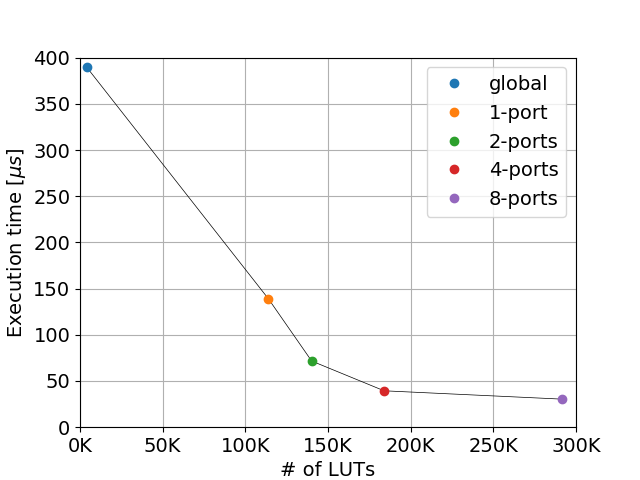
\includegraphics[width=.8\textwidth]{matmul_32_multiport_pareto}
	\caption{Pareto curve of \emph{Matrix multiplication 32x32}.}
	\label{fig:matmul_32_pareto}
\end{figure}

\clearpage

\section{Bitonic sorting}
\emph{Bitonic sorting} (Algorithm~\ref{alg:bitonic}) is a sorting algorithm
characterized by a high degree of parallelism, therefore it is suitable for
\acl{hw} implementation.

\begin{algorithm}
	\caption{\emph{Bitonic sorting} algorithm.}\label{alg:bitonic}
	\begin{algorithmic}
		\Require $a \in \mathbb{R}^N, N = 2^n$; $dir$: sorting direction
		\Ensure $a[i] \geq a[j], \forall i \geq j \wedge dir = true \vee
			a[i] \leq a[j], \forall i \geq j \wedge dir = false$
		\Procedure{Sort}{$a$, $dir$}
			\For{$b = 1, \dots, n$}
				\For{$s = i - 1, \dots, 0$}
					\For{$i = 0, \dots, N/2 - 1$}
						\State $dir_0 \gets
							(i/2^{b - 1}) \& 1$
						\State $dir_0 \gets dir_0 | dir$
						\State $step \gets 2^s$
						\State $pos \gets 2 i -
							(i \& (s - 1))$
						\State $a_0 \gets a[pos]$
						\State $a_1 \gets a[pos + step]$
						\If{$a_0 > a_1 \neq dir_0$}
							\State $tmp \gets a_0$
							\State $a_0 \gets a_1$
							\State $a_1 \gets tmp$
						\EndIf
						\State $a[pos] \gets a_0$
						\State $a[pos + step] \gets a_1$
					\EndFor
				\EndFor
			\EndFor
		\EndProcedure
	\end{algorithmic}
\end{algorithm}

From the memory accesses point of view, each inner loop iteration:
\begin{enumerate}
	\item $a[pos]$ is read.
	\item $a[pos+step]$ is read.
	\item $a[pos]$ is written.
	\item $a[pos+step]$ is written.
\end{enumerate}

The cache associated with $a$ array should be set-associative with at least 2
sets, so that the interleaved accesses to $pos$ and $pos + step$ do not
overwrite the related cache lines.

In the design under test the inner loop have been pipelined, but, due to the
data dependencies on $a$ array, the pipeline performance is limited (i.e.\
\ac{ii} is greater than 1).

Due to the multiple accesses per iteration, it is not possible to exploit:
\begin{itemize}
	\item Multiple ports: setting the number of ports to a number greater
		than one would result in a deadlock in C/\ac{rtl}
		Co-Simulation, due to scheduling issues).
	\item \texttt{get} latency tuning: due to dependencies on $a$, each
		request to \ac{l1} cache is written only when the previous
		request is read.
\end{itemize}

For these reasons the \texttt{get} latency has been fixed to 2 (not 1, because
it would lead the synthesizer to hang for unknown reasons) and the number of
ports to 1.

\subsection{128 elements}
In the case of \emph{Bitonic sorting 128}, array $a$ contains 128 elements to be
sorted ($n = 7$).
The \emph{Single-level cache configuration} is aimed at checking the performance
of the \ac{l2} cache alone, while the \emph{Multi-levels cache configuration}
has the purpose to evaluate the boost given by adding a \ac{l1} cache on top of
the \ac{l2}.

\subsubsection{Single-level cache configuration}
For the \emph{Single-level cache configuration} the cache associated with $a$ is
a fully-associative cache with two sets, so that the accesses to $pos + step$
index do not interfere with accesses to the $pos$ index.
The number of words per cache line has been kept free for design space
exploration.

Table~\ref{tab:bitonic_128_no_l1_config} summarizes the cache configuration.

\begin{table}[H]
	\begin{center}
		\begin{tabular}{ccccc}
			\hline
			\rowcolor{gray!50}
			\textbf{Sets} & \textbf{Ways} & \textbf{\ac{l1} lines} &
			\textbf{\texttt{get} latency} & \textbf{Ports} \\
			\hline
			1 & 2 & 0 & 2 & 1 \\
			\hline
		\end{tabular}
	\end{center}
	\caption{Single-level cache configuration for \emph{Bitonic sorting 128}.}
	\label{tab:bitonic_128_no_l1_config}
\end{table}

Table~\ref{tab:bitonic_128_no_l1_report} shows the achieved results, with
different number of words per cache line.
Doubling the number of words approximately doubles the resource usage, while
the performance grows at a much lower rate.

\begin{table}[H]
	\begin{center}
		\begin{tabular}{cccc}
			\hline
			\rowcolor{gray!50}
			& \textbf{8 words} & \textbf{16 words} & \textbf{32 words} \\
			\hline
			\textbf{Hit ratio} [\%] & 93.8 & 96.9 & 98.4 \\
			\rowcolor{gray!25}
			\textbf{Execution time} [$\mu s$] & 232 & 202 & 188 \\
			\textbf{\ac{bram}} & 16 & 30 & 30 \\
			\rowcolor{gray!25}
			\textbf{\acs{lut}} & 20294 & 45481 & 91656 \\
			\textbf{\acs{ff}} & 6766 & 14403 & 24851 \\
			\hline
		\end{tabular}
	\end{center}
	\caption{Performance and resource usage of \emph{Bitonic sorting 128} (single-level).}
	\label{tab:bitonic_128_no_l1_report}
\end{table}

\subsubsection{Multi-levels cache configuration}
The \emph{Multi-levels cache configuration}
(Table~\ref{tab:bitonic_128_l1_config}) matches the \emph{Single-level cache
configuration}, with the only difference that a single-line \ac{l1} cache has
been added on top of the memory hierarchy.

\begin{table}[H]
	\begin{center}
		\begin{tabular}{ccccc}
			\hline
			\rowcolor{gray!50}
			\textbf{Sets} & \textbf{Ways} & \textbf{\ac{l1} lines} &
			\textbf{\texttt{get} latency} & \textbf{Ports} \\
			\hline
			1 & 2 & 1 & 2 & 1 \\
			\hline
		\end{tabular}
	\end{center}
	\caption{Multi-levels cache configuration for \emph{Bitonic sorting 128}.}
	\label{tab:bitonic_128_l1_config}
\end{table}

Table~\ref{tab:bitonic_128_l1_report} shows some results obtained with the
\emph{Multi-levels cache configuration}. Comparing these data with the
\emph{Single-level cache configuration}
(Table~\ref{tab:bitonic_128_no_l1_report}) ones it is clear that the insertion
of the \ac{l1} cache gives a further boost to performance, without increasing
much the resource usage.

Execution time of the 16 words case is not reported because the Co-Simulation
deadlocks with that specific configuration; its value would be probably between
150 $\mu s$ and 170 $\mu s$.

\begin{table}[H]
	\begin{center}
		\begin{tabular}{cccc}
			\hline
			\rowcolor{gray!50}
			& \textbf{8 words} & \textbf{16 words} & \textbf{32 words} \\
			\hline
			\textbf{\ac{l1} hit ratio} [\%] & 16.1 & 19.6 & 22.3 \\
			\rowcolor{gray!25}
			\textbf{\ac{l2} hit ratio} [\%] & 77.7 & 77.2 & 76.1 \\
			\textbf{Execution time} [$\mu s$] & 194 & - & 130 \\
			\rowcolor{gray!25}
			\textbf{\ac{bram}} & 16 & 30 & 30 \\
			\textbf{\acs{lut}} & 20745 & 46246 & 92740 \\
			\rowcolor{gray!25}
			\textbf{\acs{ff}} & 8082 & 18025 & 33066 \\
			\hline
		\end{tabular}
	\end{center}
	\caption{Performance and resource usage of \emph{Bitonic sorting 128} (multi-levels).}
	\label{tab:bitonic_128_l1_report}
\end{table}

\subsubsection{Summary}
Table~\ref{tab:bitonic_128_report} compares the results achieved with the most
performant cache configuration (i.e.\ multi-levels with 32 words per line),
with the higher and lower bounds for performance.

Cache is almost two times faster than the global memory, but it's still one
order of magnitude slower than the local memory, and the resource usage is not
negligible.

\begin{table}[H]
	\begin{center}
		\begin{tabular}{cccc}
			\hline
			\rowcolor{gray!50}
			& \textbf{Global memory} & \textbf{Local memory} &
			\textbf{Proposed cache} \\
			\hline
			\textbf{Execution time} [$\mu s$] & 244 & 23 & 130 \\
			\rowcolor{gray!25}
			\textbf{\ac{bram}} & 2 & 30 & 30 \\
			\textbf{\acs{lut}} & 1743 & 3540 & 92740 \\
			\rowcolor{gray!25}
			\textbf{\acs{ff}} & 1088 & 3464 & 33066 \\
			\hline
		\end{tabular}
	\end{center}
	\caption{Performance and resource usage of \emph{Bitonic sorting 128}.}
	\label{tab:bitonic_128_report}
\end{table}

From Figure~\ref{fig:bitonic_128_design_space} it is easy to conclude that the
best trade-offs (between area and performance) belonging to the Pareto curve
are the ones which include the \ac{l1} cache.

\begin{figure}[H]
	\centering
	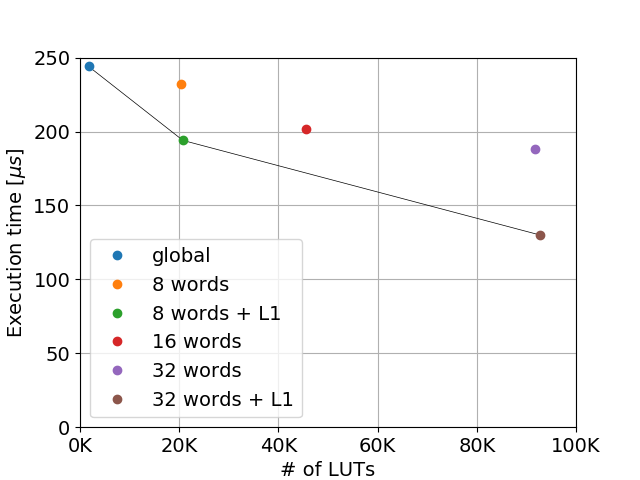
\includegraphics[width=.8\textwidth]{bitonic_design_space}
	\caption{Pareto curve of \emph{Bitonic sorting 128}.}
	\label{fig:bitonic_128_design_space}
\end{figure}

\iffalse
\subsection{1024 elements}
\subsubsection{Single-level cache configuration}
\begin{table}[H]
	\begin{center}
		\begin{tabular}{ccccc}
			\hline
			\rowcolor{gray!50}
			\textbf{Sets} & \textbf{Ways} & \textbf{\ac{l1} lines} &
			\textbf{\texttt{get} latency} & \textbf{Ports} \\
			\hline
			1 & 2 & 0 & 2 & 1 \\
			\hline
		\end{tabular}
	\end{center}
	\caption{Single-level cache configuration for \emph{Bitonic sorting 1024}.}
	\label{tab:bitonic_1024_no_l1_config}
\end{table}

\begin{table}[H]
	\begin{center}
		\begin{tabular}{cccc}
			\hline
			\rowcolor{gray!50}
			& \textbf{8 words} & \textbf{16 words} & \textbf{32 words} \\
			\hline
			\textbf{Hit ratio} [\%] & 93.8 & 96.9 & 98.4 \\
			\rowcolor{gray!25}
			\textbf{Execution time} [$\mu s$] & 3633 & 3168 & 2950 \\
			\textbf{\ac{bram}} & 16 & 30 & 30 \\
			\rowcolor{gray!25}
			\textbf{\acs{lut}} & 20342 & 45531 & 91613 \\
			\textbf{\acs{ff}} & 6806 & 14441 & 24890 \\
			\hline
		\end{tabular}
	\end{center}
	\caption{Performance and resource usage of \emph{Bitonic sorting 1024}
	(single-level).}
	\label{tab:bitonic_1024_no_l1_report}
\end{table}

\subsubsection{Multi-levels cache configuration}
\begin{table}[!htb]
	\begin{center}
		\begin{tabular}{ccccc}
			\hline
			\rowcolor{gray!50}
			\textbf{Sets} & \textbf{Ways} & \textbf{\ac{l1} lines} &
			\textbf{\texttt{get} latency} & \textbf{Ports} \\
			\hline
			1 & 2 & 1 & 2 & 1 \\
			\hline
		\end{tabular}
	\end{center}
	\caption{Multi-levels cache configuration for \emph{Bitonic sorting 1024}.}
	\label{tab:bitonic_1024_l1_config}
\end{table}

\begin{table}[H]
	\begin{center}
		\begin{tabular}{cccc}
			\hline
			\rowcolor{gray!50}
			& \textbf{8 words} & \textbf{16 words} & \textbf{32 words} \\
			\hline
			\textbf{\ac{l1} hit ratio} [\%] & 12.3 & 15.5 & 18.2 \\
			\rowcolor{gray!25}
			\textbf{\ac{l2} hit ratio} [\%] & 81.5 & 81.4 & 80.3 \\
			\textbf{Execution time} [$\mu s$] & 3190 & & 2212 \\
			\rowcolor{gray!25}
			\textbf{\ac{bram}} & 16 & 30 & 30 \\
			\textbf{\acs{lut}} & 20797 & 46304 & 92792 \\
			\rowcolor{gray!25}
			\textbf{\acs{ff}} & 8146 & 18087 & 33129 \\
			\hline
		\end{tabular}
	\end{center}
	\caption{Performance and resource usage of \emph{Bitonic sorting 1024}
	(multi-levels).}
	\label{tab:bitonic_1024_l1_report}
\end{table}

\subsubsection{Summary}
\begin{table}[H]
	\begin{center}
		\begin{tabularx}{\textwidth}{CCCCC}
			\hline
			\rowcolor{gray!50}
			& \textbf{Global memory} & \textbf{Local memory} &
			\textbf{Proposed cache (single-level)} &
			\textbf{Proposed cache (multi-levels)} \\
			\hline
			\textbf{Execution time} [$\mu s$] & 3830 & 343 &
			2950 & 2212 \\
			\rowcolor{gray!25}
			\textbf{\ac{bram}} & 2 & 32 & 30 & 30 \\
			\textbf{\acs{lut}} & 1774 & 3517 & 91613 & 92792 \\
			\rowcolor{gray!25}
			\textbf{\acs{ff}} & 1107 & 3477 & 24890 & 33129 \\
			\hline
		\end{tabularx}
	\end{center}
	\caption{Performance and resource usage of \emph{Bitonic sorting 1024}.}
	\label{tab:bitonic_1024_report}
\end{table}
\fi

\clearpage

\section{2D convolution}
Algorithm~\ref{alg:conv} is a possible implementation of \emph{2D
convolution}~\cite{conv}.

The algorithm accesses three matrices:
\begin{itemize}
	\item $A$: read according to a sliding window pattern.
	\item $kernel$: read sequentially.
	\item $B$: written sequentially.
\end{itemize}

Accesses to $kernel$ and $B$ can be optimized by single-line caches, while $A$
cache requires a more complex cache to get a sufficiently high hit ratio.

In the \acl{hw} implementation the innermost loop have been pipelined, after
moving the assignment to $B$ in its latest iteration, to make the loop nest
\emph{perfect} (i.e.\ a loop contains only another loop without any external
logic, reducing the \ac{hls} effort for pipelining).

\begin{algorithm}
	\caption{\emph{2D convolution} algorithm.}\label{alg:conv}
	\begin{algorithmic}
		\Require $A \in \mathbb{R}^{N \times M},
		kernel \in \mathbb{R}^{P \times Q}$
		\Ensure $B \in \mathbb{R}^{N \times M} : B = A \ast kernel$
		\Procedure{Conv}{$A, kernel$}
			\For{$i = 0, \dots, N - 1$}
				\For{$j = 0, \dots, M - 1$}
					\State $tmp \gets 0$
					\For{$m = 0, \dots, P - 1$}
						\For{$n = 0, \dots, Q - 1$}
							\State $ii \gets
								i + (Q / 2 - m)$
							\State $jj \gets
								j + (P / 2 - n)$

							\If{$ii \geq 0 \And
									ii < N \And
									jj \geq 0 \And
									jj < M$}
								\State $tmp \gets
									tmp + A[ii][jj] \cdot
									kernel[m][n]$
							\EndIf
						\EndFor
					\EndFor
					\State $B[i][j] \gets tmp$
				\EndFor
			\EndFor
		\EndProcedure
	\end{algorithmic}
\end{algorithm}

\subsection{32x32 matrix and 9x9 kernel}
The design under test has been set such that $A, B \in \mathbb{N}^{32 \times
32}$ and the $kernel \in \mathbb{N}^{3 \times 3}$.

The cache associated with $A$ matrix is fully associative with 4 sets, to ensure
that consecutive cache accesses do not overwrite previously loaded line.
The other parameters have been left free for design space exploration.

$kernel$ cache has been set to work as a line buffer: it contains a single line
which fits the whole kernel, so that the first request load the kernel to cache
and all the subsequent accesses are \ac{l1} cache hits.

$B$ cache has the purpose of gathering multiple write requests.

The full configuration of caches is shown in Table~\ref{tab:conv_cache_config}.

\begin{table}[H]
	\begin{center}
		\begin{tabular}{cccccc}
			\hline
			\rowcolor{gray!50}
			\textbf{Matrix} & \textbf{Sets} & \textbf{Ways} &
			\textbf{Words per line} & \textbf{\ac{l1} lines} &
			\textbf{Hit ratio} [\%] \\
			\hline
			$A$ & 1 & 4 & Free & Free & ? \\
			\rowcolor{gray!25}
			$kernel$ & 1 & 1 & 16 & 1 & 100 \\
			$B$ & 1 & 1 & 32 & 0 & 96.9 \\
			\hline
		\end{tabular}
	\end{center}
	\caption{$kernel$ and $B$ caches configuration for \emph{2D convolution}.}
	\label{tab:conv_cache_config}
\end{table}

\subsubsection{Single-level cache configuration}
With the \emph{Single-level cache configuration} the $A$ cache is configured to
have no \ac{l1} cache, while the number of words per line is kept free.
The \texttt{get} latency has been set to 9 for both $A$ and $kernel$ caches.

Table~\ref{tab:conv_no_l1_report} reports the collected results.
The execution time with 32 words is missing since this configuration causes a
deadlock in Co-Simulation.

\begin{table}[H]
	\begin{center}
		\begin{tabular}{cccc}
			\hline
			\rowcolor{gray!50}
			& \textbf{8 words} & \textbf{16 words} & \textbf{32 words} \\
			\hline
			\textbf{$A$ hit ratio} [\%] & 89.6 & 95.8 & 99.6 \\
			\rowcolor{gray!25}
			\textbf{Execution time} [$\mu s$] & 45 & 40 & - \\
			\textbf{\ac{bram}} & 146 & 174 & 174 \\
			\rowcolor{gray!25}
			\textbf{\ac{dsp}} & 3 & 3 & 3 \\
			\textbf{\acs{lut}} & 85574 & 91190 & 102887 \\
			\rowcolor{gray!25}
			\textbf{\acs{ff}} & 33803 & 37779 & 44578 \\
			\hline
		\end{tabular}
	\end{center}
	\caption{Performance and resource usage of \emph{2D convolution}
	(single-level).}
	\label{tab:conv_no_l1_report}
\end{table}

\subsubsection{Multi-levels cache configuration}
The \emph{Multi-levels cache configuration} is equivalent to the
\emph{Single-level}, but a single-line \ac{l1} cache has been added.

The performance advantage with respect to the \emph{Single-level configuration}
is negligible, therefore it is not convenient to invest in more resources in
this case.

\begin{table}[H]
	\begin{center}
		\begin{tabular}{cccc}
			\hline
			\rowcolor{gray!50}
			& \textbf{8 words} & \textbf{16 words} & \textbf{32 words} \\
			\hline
			\textbf{$A$ \ac{l1} hit ratio} [\%] & 59.6 & 63.8 & 66.0 \\
			\rowcolor{gray!25}
			\textbf{$A$ \ac{l2} hit ratio} [\%] & 30.1 & 32.0 & 33.7 \\
			\textbf{Execution time} [$\mu s$] & 43 & 40 & 39 \\
			\rowcolor{gray!25}
			\textbf{\ac{bram}} & 146 & 174 & 174 \\
			\textbf{\ac{dsp}} & 3 & 3 & 3 \\
			\rowcolor{gray!25}
			\textbf{\acs{lut}} & 85640 & 91274 & 102970 \\
			\textbf{\acs{ff}} & 40288 & 50146 & 68720 \\
			\hline
		\end{tabular}
	\end{center}
	\caption{Performance and resource usage of \emph{2D convolution}
	(multi-levels).}
	\label{tab:conv_l1_report}
\end{table}

\subsubsection{Summary}
Table~\ref{tab:conv_report} compares the most performant cache configuration
(i.e.\ multi-levels with 32 words per line) with the performance bounds: the
achieved performance is almost equal to the performance higher bound.

\begin{table}[H]
	\begin{center}
		\begin{tabular}{cccc}
			\hline
			\rowcolor{gray!50}
			& \textbf{Global memory} & \textbf{Local memory} &
			\textbf{Cache} \\
			\hline
			\textbf{Execution time} [$\mu s$] & 66 & 37 & 39 \\
			\rowcolor{gray!25}
			\textbf{\ac{bram}} & 12 & 178 & 174 \\
			\textbf{\acs{dsp}} & 3 & 3 & 3 \\
			\rowcolor{gray!25}
			\textbf{\acs{lut}} & 3504 & 30897 & 102970 \\
			\textbf{\acs{ff}} & 3257 & 10672 & 68720 \\
			\hline
		\end{tabular}
	\end{center}
	\caption{Performance and resource usage of \emph{Convolution}.}
	\label{tab:conv_report}
\end{table}

The plot shown in Figure~\ref{fig:conv_design_space} suggests that the
single-level 16 words per line configuration may be the most convenient in this
case, since it offers almost the same performance and requires almost half of
the \acp{ff} with respect to the multi-levels 32 words configuration.

\begin{figure}[H]
	\centering
	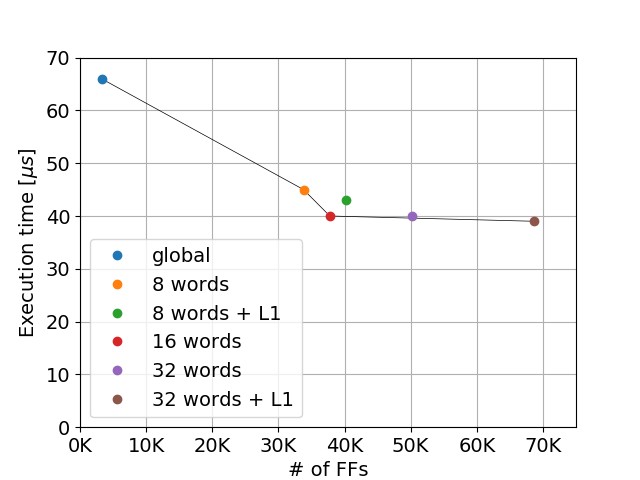
\includegraphics[width=.8\textwidth]{conv_design_space}
	\caption{Pareto curve of \emph{2D convolution}.}
	\label{fig:conv_design_space}
\end{figure}

\chapter{Conclusions}
This thesis work proven the possibility to implement multi-process designs in
\ac{hls}.

The cache process itself can provide high performance thanks to its optimal
pipelining (i.e. \ac{ii} of 1), but some issues arise from the proposed
\acl{ipc} protocol: \emph{Vitis~HLS~2021.1} do not provide any mechanism to
inform the scheduler about the dependencies and latency between the request
writing to a \ac{fifo} and the response reading from another \ac{fifo},
therefore the accesses to these data structures are not optimally scheduled by
\ac{hls}, resulting in performance loss and in some cases even deadlocks.

The proposed workaround of forcing clock cycles to increase the latency between
the \ac{fifo} write and the \ac{fifo} read allows to achieve optimal results in
some specific situations, but it can not always work.

\bigskip
The collected results prove that in general the resource usage required by the
proposed cache module is paid off in terms of performance, without requiring
high design efforts for optimizing memory interfacing: it is enough to include
the cache in the kernel and setup the parameters according to the desired
performance and resource usage.

In some cases it is possible to achieve very high performance gain (e.g.\
\emph{Matrix multiplication} achieved a reduction of execution time of more
than one order of magnitude).

\bigskip
To overcome the limitations posed by the \ac{hls} tool it may be worth
implementing the interface with the cache or the whole architecture at
\ac{rtl}, which provides full control on the operations scheduling.

The cache performance could be further improved by implementing a pre-fetching
mechanism which analyses the memory access patterns and tries to load in advance
the data, before it is requested.

\backmatter

\printbibliography

\end{document}

